\documentclass[12pt,a4paper]{article}
\usepackage[brazil]{babel}
\usepackage{fontspec}
% fontes pelo nome do arquivo (o Tectonic as traz no pacote, mas não pelo nome da família)
\setmainfont{texgyretermes}[Extension=.otf,UprightFont=*-regular,BoldFont=*-bold,ItalicFont=*-italic,BoldItalicFont=*-bolditalic]
\setsansfont{texgyreheros}[Extension=.otf,UprightFont=*-regular,BoldFont=*-bold,ItalicFont=*-italic,BoldItalicFont=*-bolditalic]
\setmonofont{texgyrecursor}[Scale=0.92,Extension=.otf,UprightFont=*-regular,BoldFont=*-bold,ItalicFont=*-italic,BoldItalicFont=*-bolditalic]
\usepackage{amssymb,newunicodechar}
\newunicodechar{≤}{\ensuremath{\leq}}
\newunicodechar{→}{\ensuremath{\rightarrow}}
\newunicodechar{✓}{\ensuremath{\checkmark}}
\usepackage[a4paper,top=110pt,bottom=95pt,left=85pt,right=80pt,headheight=14pt,footskip=40pt]{geometry}
\usepackage[table]{xcolor}
\definecolor{azul}{HTML}{1F3864}
\definecolor{cinzarodape}{HTML}{6B809B}
\definecolor{linhapar}{HTML}{F2F5FA}
\definecolor{bordatab}{HTML}{B4B4B4}
\arrayrulecolor{bordatab}
\usepackage{graphicx,eso-pic,fancyhdr,longtable,array,enumitem,setspace,placeins,microtype}
\usepackage[explicit]{titlesec}
\usepackage{tocloft}
\usepackage[hidelinks]{hyperref}

\setstretch{1.15}
\setlength{\parindent}{0pt}
\setlength{\parskip}{6pt}
\setlength{\emergencystretch}{2em}
\renewcommand{\arraystretch}{1.25}
\setlist[itemize]{label=\textbullet,leftmargin=20pt,itemsep=3pt,topsep=2pt}

% títulos (a numeração já vem no texto)
\titleformat{\section}{\color{azul}\bfseries\fontsize{16}{19}\selectfont}{}{0pt}{#1}
\titleformat{\subsection}{\color{azul}\bfseries\fontsize{13}{16}\selectfont}{}{0pt}{#1}
\titleformat{\subsubsection}{\bfseries\normalsize}{}{0pt}{#1}
\titlespacing*{\section}{0pt}{6pt}{10pt}
\titlespacing*{\subsection}{0pt}{12pt}{6pt}
\titlespacing*{\subsubsection}{0pt}{9pt}{4pt}

% índice
\addto\captionsbrazil{\renewcommand{\contentsname}{Índice}}
\renewcommand{\cfttoctitlefont}{\color{azul}\bfseries\fontsize{16}{19}\selectfont}
\renewcommand{\cftsecleader}{\cftdotfill{\cftdotsep}}
\renewcommand{\cftsecfont}{\normalfont}
\renewcommand{\cftsecpagefont}{\normalfont}
\setlength{\cftsubsecindent}{18pt}
\setlength{\cftbeforesecskip}{3pt}

% figuras: legenda em itálico, centralizada (o texto já traz "Figura N –")
\newcommand{\legenda}[1]{\par\vspace{4pt}{\small\itshape #1\par}}
\renewcommand{\topfraction}{0.95}
\renewcommand{\bottomfraction}{0.6}
\renewcommand{\textfraction}{0.05}
\renewcommand{\floatpagefraction}{0.75}
\setlength{\textfloatsep}{14pt plus 4pt minus 2pt}
\setlength{\floatsep}{12pt plus 4pt minus 2pt}

% hierarquias em fonte mono, recuadas
\newenvironment{hierarquias}{\par\nopagebreak\leftskip=20pt\small\setlength{\parskip}{0pt}}{\par\medskip}

% template do ICMC: faixa lateral e logo (posições em pt medidas no PDF do enunciado)
\AddToShipoutPictureBG{\AtPageUpperLeft{%
  \put(5,-837.9){
\includegraphics[width=69.8pt,height=831.9pt]{figuras/faixa.png}}%
  \put(73.6,-85.5){
\includegraphics[width=522.6pt,height=63.6pt]{figuras/header.png}}}}
\newcommand{\rodapeicmc}{{\sffamily\fontsize{8}{10}\selectfont\color{cinzarodape}Av. Trabalhador São-carlense, 400 . centro . São Carlos - SP . cep 13566-590 . Brasil . www.icmc.usp.br}}
\fancypagestyle{icmc}{\fancyhf{}\renewcommand{\headrulewidth}{0pt}%
  \fancyfoot[C]{\hfill{\sffamily\fontsize{8}{10}\selectfont\color{cinzarodape}\thepage}\\[3pt]\rodapeicmc}}
\fancypagestyle{capa}{\fancyhf{}\renewcommand{\headrulewidth}{0pt}\fancyfoot[C]{\rodapeicmc}}
\pagestyle{icmc}
\begin{document}
\begin{titlepage}\thispagestyle{capa}\centering\setstretch{1.1}
\vspace*{10pt}
{\bfseries Departamento de Ciências de Computação – SCC\\
Instituto de Ciências Matemáticas e de Computação – ICMC\\
Universidade de São Paulo – USP\\
Disciplina SCC0245 – Processamento Analítico de Dados\\[10pt]
Docente Responsável: Profa. Cristina Dutra de Aguiar\par}
\vspace{60pt}
{\bfseries\fontsize{13}{16}\selectfont Trabalho Prático 1\par}\vspace{10pt}
{\color{azul}\bfseries\fontsize{18}{22}\selectfont Data Warehouse para Análise da Cobertura da\\ Atenção Primária a Saúde em São Carlos\par}\vspace{8pt}
{\itshape Unidades e equipes de saúde, demanda ambulatorial e internações evitáveis\par}
\vspace{60pt}
{\arrayrulecolor{gray}\renewcommand{\arraystretch}{1.5}
\begin{tabular}{|p{0.62\linewidth}|p{0.22\linewidth}|}\hline
\rowcolor[HTML]{E8EDF5}\textbf{Integrante} & \textbf{Nº USP} \\ \hline
Ivan Sardon Medina & [Nº USP] \\ \hline
Vinícius Morotti & [Nº USP] \\ \hline
Germano Antonio Zani Jorge & [Nº USP] \\ \hline
Matheus Rodrigues & [Nº USP] \\ \hline
\end{tabular}\par}
\vfill
São Carlos, 29 de Outubro de 2026\par
\vspace{30pt}
\end{titlepage}
\setcounter{page}{2}\tableofcontents\clearpage

\FloatBarrier\section*{1. Descrição do Problema}\addcontentsline{toc}{section}{1. Descrição do Problema}

\FloatBarrier\subsection*{1.1 Tema geral do trabalho}\addcontentsline{toc}{subsection}{1.1 Tema geral do trabalho}

O tema do trabalho é a \textbf{cobertura da atenção básica (Atenção Primária à Saúde – APS) no município de São Carlos (SP)}, analisada a partir de três ângulos complementares: a \textbf{oferta} de equipes de saúde, a \textbf{demanda} por atendimentos ambulatoriais e as \textbf{internações hospitalares evitáveis}. O trabalho se insere na temática da disciplina de apoio à formulação de políticas públicas municipais e utiliza exclusivamente dados reais e oficiais do Sistema Único de Saúde (SUS) e do IBGE.


A atenção básica é a porta de entrada do SUS: são as Unidades Básicas de Saúde (UBS) e as Unidades de Saúde da Família (USF), com suas equipes de Saúde da Família (eSF) e de Atenção Primária (eAP), que acompanham a população de um território. Quando esse acompanhamento funciona, problemas como hipertensão, diabetes, asma ou infecções urinárias são controlados no posto de saúde. Quando falha, eles evoluem e acabam em internações hospitalares, que são mais caras para o município e piores para o paciente. Essas internações são chamadas de \textbf{Internações por Condições Sensíveis à Atenção Primária (ICSAP)} e têm uma lista oficial definida pela Portaria SAS/MS nº 221/2008. A taxa de ICSAP é um dos indicadores mais usados para avaliar a efetividade da atenção básica.


A \textbf{importância} do tema para a gestão municipal está em responder perguntas concretas: quantas equipes de atenção básica o município mantém ao longo do tempo e onde elas estão; que tipo de atendimento ambulatorial a rede realiza; quais internações da população são evitáveis, em que grupos da população e por quais causas; e se variações na oferta de equipes acompanham variações nas internações evitáveis. As respostas apoiam decisões como abrir ou reforçar equipes, priorizar linhas de cuidado (por exemplo, hipertensão e diabetes em idosos) e acompanhar o efeito dessas políticas.


\FloatBarrier\subsection*{1.2 Fontes de dados}\addcontentsline{toc}{subsection}{1.2 Fontes de dados}

O data warehouse é povoado por cinco fontes, todas públicas e oficiais. As três primeiras são as principais e vêm do DATASUS (Departamento de Informática do SUS), obtidas com a biblioteca PySUS; as duas últimas são fontes auxiliares usadas para enriquecer e integrar as dimensões.


{\small\rowcolors{2}{white}{linhapar}\begin{longtable}{|>{\raggedright\arraybackslash}p{\dimexpr0.2638\linewidth-2\tabcolsep-1.33\arrayrulewidth\relax}|>{\raggedright\arraybackslash}p{\dimexpr0.4172\linewidth-2\tabcolsep-1.33\arrayrulewidth\relax}|>{\raggedright\arraybackslash}p{\dimexpr0.3190\linewidth-2\tabcolsep-1.33\arrayrulewidth\relax}|}\hline\rowcolor{azul}\color{white}\bfseries Fonte & \color{white}\bfseries Conteúdo & \color{white}\bfseries Uso no DW \\ \hline\endhead
CNES – Cadastro Nacional de Estabelecimentos de Saúde, arquivos EP (equipes) e ST (estabelecimentos) & Equipes de saúde cadastradas em cada estabelecimento, com tipo e datas de ativação e desativação; características dos estabelecimentos (tipo de unidade, gestão, município) & Fato de equipes; dimensões de estabelecimento e tipo de equipe \\ \hline
SIH-SUS – Sistema de Informações Hospitalares, arquivo RD (AIH reduzida) & Uma linha por Autorização de Internação Hospitalar: paciente (sexo, idade, município de residência), hospital, diagnóstico, procedimento, dias de permanência, valor & Fato de internações; dimensões de diagnóstico, procedimento, perfil do paciente, localidade e bugiganga \\ \hline
SIA-SUS – Sistema de Informações Ambulatoriais, arquivo PA (produção ambulatorial) & Produção ambulatorial por estabelecimento, procedimento, competência, ocupação do profissional (CBO) e perfil do paciente; quantidades e valores apresentados e aprovados & Fato de produção ambulatorial; dimensões de procedimento, perfil, localidade e CBO \\ \hline
IBGE – API de Localidades & Municípios de SP com código de 7 dígitos, nome, região imediata e região intermediária & Nomes e hierarquia geográfica das dimensões de localidade e estabelecimento \\ \hline
Ministério da Saúde – API de Dados Abertos (CNES) & Nome fantasia, bairro e coordenadas de cada estabelecimento & Atributos descritivos da dimensão de estabelecimento \\ \hline\end{longtable}}

\textbf{Recorte.} O período analisado vai de janeiro de 2023 a dezembro de 2024 (24 competências mensais). Os arquivos do DATASUS são estaduais; do estado de São Paulo são mantidos apenas os registros ligados a São Carlos: equipes sediadas no município, e internações e atendimentos de pacientes \textbf{residentes} em São Carlos ou \textbf{atendidos} em São Carlos. Manter os dois critérios permite analisar tanto a população do município (que às vezes é internada em outras cidades) quanto a rede instalada no município (que também atende moradores da região).


\FloatBarrier\subsection*{1.3 Processos de negócio}\addcontentsline{toc}{subsection}{1.3 Processos de negócio}

Foram modelados três processos de negócio (assuntos de interesse), cada um dando origem a uma tabela de fatos.


\subsubsection*{Processo 1 – Oferta de equipes da atenção básica}

\textbf{Descrição e justificativa.} Mede a capacidade instalada da atenção básica: quantas equipes estão ativas, de que tipo e em quais estabelecimentos. É a variável de política pública mais diretamente controlada pelo gestor municipal.


\begin{itemize}\item \textbf{Grão:} uma equipe ativa em um estabelecimento em um mês (fotografia mensal, ou \textit{snapshot} periódico).
\item \textbf{Dimensões:} tempo (mês), estabelecimento, tipo de equipe. O identificador da equipe é guardado como dimensão degenerada.
\item \textbf{Fatos:} não há medida numérica armazenada; trata-se de uma \textbf{tabela de fatos sem fato}. O número de equipes é obtido contando as linhas. Essa contagem é \textbf{semiaditiva}: pode ser somada entre estabelecimentos e tipos de equipe, mas não ao longo do tempo (somar as equipes de janeiro e de fevereiro contaria a mesma equipe duas vezes). Ao agregar vários meses, usa-se a média mensal ou o valor do último mês.\end{itemize}

\subsubsection*{Processo 2 – Internações hospitalares}

\textbf{Descrição e justificativa.} Registra cada internação paga pelo SUS. Permite identificar as internações sensíveis à atenção primária, que funcionam como sinal de falha da rede básica, e caracterizá-las por causa, faixa etária, sexo e hospital.


\begin{itemize}\item \textbf{Grão:} uma internação (uma AIH).
\item \textbf{Dimensões:} tempo, estabelecimento (hospital), procedimento realizado, diagnóstico principal, perfil do paciente, localidade de residência do paciente e tabela bugiganga (caráter do atendimento, óbito, uso de UTI). O número da AIH é dimensão degenerada.
\item \textbf{Fatos:} quantidade de internações (sempre 1 por linha, \textbf{aditivo}), dias de permanência (\textbf{aditivo}) e valor total pago em reais (\textbf{aditivo}). A média de permanência é um fato \textbf{derivado e não aditivo}, obtido pela soma dos dias dividida pela quantidade de internações.\end{itemize}

\subsubsection*{Processo 3 – Produção ambulatorial}

\textbf{Descrição e justificativa.} Mede a demanda atendida nos ambulatórios do SUS: consultas, exames, procedimentos e ações de prevenção. Mostra o volume e o tipo de atendimento que a rede realiza e o perfil de quem é atendido.


\begin{itemize}\item \textbf{Grão:} estabelecimento × procedimento × mês × perfil do paciente (sexo e faixa etária) × município de residência × ocupação do profissional. É o menor nível de detalhe disponível no arquivo público do SIA, que já vem parcialmente agregado.
\item \textbf{Dimensões:} tempo, estabelecimento, procedimento, perfil do paciente, localidade de residência, ocupação (CBO).
\item \textbf{Fatos:} quantidade apresentada, quantidade aprovada, valor apresentado e valor aprovado, todos \textbf{aditivos}. A taxa de aprovação é um fato \textbf{derivado e não aditivo}: quantidade aprovada dividida pela quantidade apresentada, calculada sempre sobre as somas e nunca somando taxas.\end{itemize}

\subsubsection*{Medidas derivadas entre processos}

\begin{itemize}\item \textbf{Cobertura estimada de Saúde da Família (\%)} = número de equipes eSF × 3.450 pessoas ÷ população do município × 100, limitada a 100\%. O parâmetro de 3.450 pessoas por equipe é o usado historicamente pelo Ministério da Saúde. Não aditiva.
\item \textbf{Taxa de ICSAP por 10 mil habitantes} = internações ICSAP de residentes ÷ população × 10.000. Não aditiva.
\item A população usada é a do Censo 2022 do IBGE para São Carlos (254.857 habitantes).\end{itemize}

\FloatBarrier\subsection*{1.4 Dimensões e seus atributos}\addcontentsline{toc}{subsection}{1.4 Dimensões e seus atributos}

Todas as dimensões usam uma \textbf{chave artificial} (\textit{surrogate key}, prefixo \texttt{sk\_\allowbreak{}}) como chave primária, independente dos códigos das fontes. Cada dimensão também tem um membro de chave 0, “Não informado”, que recebe os fatos cujo código não é encontrado, para que nenhum registro seja perdido na carga. Nas tabelas abaixo, a coluna “Relação” indica se o atributo participa de uma hierarquia ou é apenas descritivo.


\subsubsection*{dim\_\allowbreak{}tempo}

Mês de competência, isto é, o mês a que o registro se refere no sistema do Ministério da Saúde. Todas as fontes são mensais, então o mês é o menor nível de detalhe comum.


{\small\rowcolors{2}{white}{linhapar}\begin{longtable}{|>{\raggedright\arraybackslash}p{\dimexpr0.2209\linewidth-2\tabcolsep-1.25\arrayrulewidth\relax}|>{\raggedright\arraybackslash}p{\dimexpr0.3067\linewidth-2\tabcolsep-1.25\arrayrulewidth\relax}|>{\raggedright\arraybackslash}p{\dimexpr0.1963\linewidth-2\tabcolsep-1.25\arrayrulewidth\relax}|>{\raggedright\arraybackslash}p{\dimexpr0.2761\linewidth-2\tabcolsep-1.25\arrayrulewidth\relax}|}\hline\rowcolor{azul}\color{white}\bfseries Atributo & \color{white}\bfseries Significado & \color{white}\bfseries Relação & \color{white}\bfseries Povoamento (fonte) \\ \hline\endhead
sk\_\allowbreak{}tempo & Chave artificial & – & Gerada na carga \\ \hline
ano\_\allowbreak{}mes & Competência no formato AAAAMM & Hierarquia (nível mais baixo) & SIH: ANO\_\allowbreak{}CMPT + MES\_\allowbreak{}CMPT; SIA: PA\_\allowbreak{}MVM; CNES: COMPETEN (integração) \\ \hline
mes & Número do mês (1 a 12) & Descritivo & Derivado de ano\_\allowbreak{}mes \\ \hline
nome\_\allowbreak{}mes & Nome abreviado do mês & Descritivo & Derivado de ano\_\allowbreak{}mes \\ \hline
trimestre & Trimestre do ano (ex.: 2024-T1) & Hierarquia & Derivado de ano\_\allowbreak{}mes \\ \hline
semestre & Semestre do ano (ex.: 2024-S1) & Hierarquia & Derivado de ano\_\allowbreak{}mes \\ \hline
ano & Ano & Hierarquia (nível mais alto) & Derivado de ano\_\allowbreak{}mes \\ \hline\end{longtable}}

\subsubsection*{dim\_\allowbreak{}estabelecimento}

Estabelecimento de saúde (UBS, USF, hospital, clínica, pronto atendimento etc.), identificado pelo código CNES. É compartilhada pelos três processos.


{\small\rowcolors{2}{white}{linhapar}\begin{longtable}{|>{\raggedright\arraybackslash}p{\dimexpr0.2209\linewidth-2\tabcolsep-1.25\arrayrulewidth\relax}|>{\raggedright\arraybackslash}p{\dimexpr0.3067\linewidth-2\tabcolsep-1.25\arrayrulewidth\relax}|>{\raggedright\arraybackslash}p{\dimexpr0.1963\linewidth-2\tabcolsep-1.25\arrayrulewidth\relax}|>{\raggedright\arraybackslash}p{\dimexpr0.2761\linewidth-2\tabcolsep-1.25\arrayrulewidth\relax}|}\hline\rowcolor{azul}\color{white}\bfseries Atributo & \color{white}\bfseries Significado & \color{white}\bfseries Relação & \color{white}\bfseries Povoamento (fonte) \\ \hline\endhead
sk\_\allowbreak{}estabelecimento & Chave artificial & – & Gerada na carga \\ \hline
cnes & Código nacional do estabelecimento, 7 dígitos (chave natural) & Hierarquia (nível mais baixo) & CNES, SIH (CNES) e SIA (PA\_\allowbreak{}CODUNI), padronizado com zeros à esquerda \\ \hline
nome & Nome fantasia & Descritivo & API de Dados Abertos (nome\_\allowbreak{}fantasia) \\ \hline
tipo\_\allowbreak{}unidade\_\allowbreak{}cod / tipo\_\allowbreak{}unidade & Tipo do estabelecimento (ex.: 02 – Centro de saúde / Unidade básica) & Hierarquia & CNES-ST (TP\_\allowbreak{}UNID); na falta, API (codigo\_\allowbreak{}tipo\_\allowbreak{}unidade) \\ \hline
nivel\_\allowbreak{}atencao & Atenção Primária, Especializada, Hospitalar, Urgência ou Outros & Hierarquia & Derivado do tipo de unidade \\ \hline
gestao & Gestão municipal, estadual ou dupla & Descritivo & CNES-ST (TPGESTAO) \\ \hline
bairro & Bairro do estabelecimento & Hierarquia & API de Dados Abertos \\ \hline
latitude / longitude & Coordenadas geográficas & Descritivos & API de Dados Abertos \\ \hline
cod\_\allowbreak{}municipio / municipio & Município do estabelecimento & Hierarquia & CNES-ST (CODUFMUN) + nome do IBGE \\ \hline
regiao\_\allowbreak{}imediata & Região geográfica imediata do IBGE & Hierarquia & IBGE \\ \hline
uf & Unidade da federação & Hierarquia (nível mais alto) & IBGE / prefixo do código do município \\ \hline\end{longtable}}

\subsubsection*{dim\_\allowbreak{}localidade}

Município de residência do paciente. Permite separar a população de São Carlos dos pacientes de outras cidades atendidos no município.


{\small\rowcolors{2}{white}{linhapar}\begin{longtable}{|>{\raggedright\arraybackslash}p{\dimexpr0.2209\linewidth-2\tabcolsep-1.25\arrayrulewidth\relax}|>{\raggedright\arraybackslash}p{\dimexpr0.3067\linewidth-2\tabcolsep-1.25\arrayrulewidth\relax}|>{\raggedright\arraybackslash}p{\dimexpr0.1963\linewidth-2\tabcolsep-1.25\arrayrulewidth\relax}|>{\raggedright\arraybackslash}p{\dimexpr0.2761\linewidth-2\tabcolsep-1.25\arrayrulewidth\relax}|}\hline\rowcolor{azul}\color{white}\bfseries Atributo & \color{white}\bfseries Significado & \color{white}\bfseries Relação & \color{white}\bfseries Povoamento (fonte) \\ \hline\endhead
sk\_\allowbreak{}localidade & Chave artificial & – & Gerada na carga \\ \hline
cod\_\allowbreak{}municipio & Código do município, 6 dígitos & Hierarquia (nível mais baixo) & SIH (MUNIC\_\allowbreak{}RES), SIA (PA\_\allowbreak{}MUNPCN), IBGE (7 dígitos convertidos) \\ \hline
municipio & Nome do município & Descritivo do nível município & IBGE \\ \hline
regiao\_\allowbreak{}imediata & Região imediata do IBGE (ex.: São Carlos) & Hierarquia & IBGE \\ \hline
regiao\_\allowbreak{}intermediaria & Região intermediária do IBGE (ex.: Araraquara) & Hierarquia & IBGE \\ \hline
uf & Unidade da federação & Hierarquia (nível mais alto) & IBGE / prefixo do código \\ \hline\end{longtable}}

\subsubsection*{dim\_\allowbreak{}tipo\_\allowbreak{}equipe}

Tipo da equipe de saúde, conforme a classificação do CNES.


{\small\rowcolors{2}{white}{linhapar}\begin{longtable}{|>{\raggedright\arraybackslash}p{\dimexpr0.2209\linewidth-2\tabcolsep-1.25\arrayrulewidth\relax}|>{\raggedright\arraybackslash}p{\dimexpr0.3067\linewidth-2\tabcolsep-1.25\arrayrulewidth\relax}|>{\raggedright\arraybackslash}p{\dimexpr0.1963\linewidth-2\tabcolsep-1.25\arrayrulewidth\relax}|>{\raggedright\arraybackslash}p{\dimexpr0.2761\linewidth-2\tabcolsep-1.25\arrayrulewidth\relax}|}\hline\rowcolor{azul}\color{white}\bfseries Atributo & \color{white}\bfseries Significado & \color{white}\bfseries Relação & \color{white}\bfseries Povoamento (fonte) \\ \hline\endhead
sk\_\allowbreak{}tipo\_\allowbreak{}equipe & Chave artificial & – & Gerada na carga \\ \hline
tipo\_\allowbreak{}equipe\_\allowbreak{}cod & Código do tipo (ex.: 70) & Hierarquia (nível mais baixo) & CNES-EP (TIPO\_\allowbreak{}EQP) \\ \hline
tipo\_\allowbreak{}equipe & Descrição (ex.: eSF – Equipe de Saúde da Família) & Descritivo do código & Tabela de tipos de equipe do CNES \\ \hline
categoria\_\allowbreak{}equipe & Saúde da Família, Atenção Primária, Saúde Bucal, Multiprofissional ou Outras & Hierarquia (nível mais alto) & Classificação definida pelo grupo \\ \hline\end{longtable}}

\subsubsection*{dim\_\allowbreak{}procedimento}

Procedimento da Tabela de Procedimentos do SUS (SIGTAP), usada tanto pelo SIA quanto pelo SIH. O próprio código de 10 dígitos é hierárquico.


{\small\rowcolors{2}{white}{linhapar}\begin{longtable}{|>{\raggedright\arraybackslash}p{\dimexpr0.2209\linewidth-2\tabcolsep-1.25\arrayrulewidth\relax}|>{\raggedright\arraybackslash}p{\dimexpr0.3067\linewidth-2\tabcolsep-1.25\arrayrulewidth\relax}|>{\raggedright\arraybackslash}p{\dimexpr0.1963\linewidth-2\tabcolsep-1.25\arrayrulewidth\relax}|>{\raggedright\arraybackslash}p{\dimexpr0.2761\linewidth-2\tabcolsep-1.25\arrayrulewidth\relax}|}\hline\rowcolor{azul}\color{white}\bfseries Atributo & \color{white}\bfseries Significado & \color{white}\bfseries Relação & \color{white}\bfseries Povoamento (fonte) \\ \hline\endhead
sk\_\allowbreak{}procedimento & Chave artificial & – & Gerada na carga \\ \hline
cod\_\allowbreak{}procedimento & Código de 10 dígitos & Hierarquia (nível mais baixo) & SIA (PA\_\allowbreak{}PROC\_\allowbreak{}ID), SIH (PROC\_\allowbreak{}REA) \\ \hline
forma\_\allowbreak{}organizacao\_\allowbreak{}cod & 6 primeiros dígitos & Hierarquia & Derivado do código \\ \hline
subgrupo\_\allowbreak{}cod & 4 primeiros dígitos & Hierarquia & Derivado do código \\ \hline
grupo\_\allowbreak{}cod / grupo & 2 primeiros dígitos e nome do grupo (ex.: 03 – Procedimentos clínicos) & Hierarquia (nível mais alto) & Derivado do código + SIGTAP \\ \hline\end{longtable}}

\subsubsection*{dim\_\allowbreak{}diagnostico}

Diagnóstico principal da internação segundo a CID-10, com a classificação de condição sensível à atenção primária.


{\small\rowcolors{2}{white}{linhapar}\begin{longtable}{|>{\raggedright\arraybackslash}p{\dimexpr0.2209\linewidth-2\tabcolsep-1.25\arrayrulewidth\relax}|>{\raggedright\arraybackslash}p{\dimexpr0.3067\linewidth-2\tabcolsep-1.25\arrayrulewidth\relax}|>{\raggedright\arraybackslash}p{\dimexpr0.1963\linewidth-2\tabcolsep-1.25\arrayrulewidth\relax}|>{\raggedright\arraybackslash}p{\dimexpr0.2761\linewidth-2\tabcolsep-1.25\arrayrulewidth\relax}|}\hline\rowcolor{azul}\color{white}\bfseries Atributo & \color{white}\bfseries Significado & \color{white}\bfseries Relação & \color{white}\bfseries Povoamento (fonte) \\ \hline\endhead
sk\_\allowbreak{}diagnostico & Chave artificial & – & Gerada na carga \\ \hline
cid & Código CID-10 com 4 caracteres (ex.: J181) & Hierarquia (nível mais baixo) & SIH (DIAG\_\allowbreak{}PRINC) \\ \hline
cid\_\allowbreak{}categoria & 3 primeiros caracteres (ex.: J18) & Hierarquia & Derivado do código \\ \hline
capitulo\_\allowbreak{}num / capitulo & Capítulo da CID-10 (ex.: X – Aparelho respiratório) & Hierarquia & Tabela da CID-10 \\ \hline
grupo\_\allowbreak{}icsap & Um dos 19 grupos de ICSAP ou “Não ICSAP” & Hierarquia & Portaria SAS/MS nº 221/2008 \\ \hline
icsap & Sim / Não & Hierarquia (nível mais alto) & Derivado de grupo\_\allowbreak{}icsap \\ \hline\end{longtable}}

\subsubsection*{dim\_\allowbreak{}perfil\_\allowbreak{}paciente}

Perfil demográfico do paciente. É uma mini-dimensão com todas as combinações de sexo e faixa etária, compartilhada pelos processos 2 e 3.


{\small\rowcolors{2}{white}{linhapar}\begin{longtable}{|>{\raggedright\arraybackslash}p{\dimexpr0.2209\linewidth-2\tabcolsep-1.25\arrayrulewidth\relax}|>{\raggedright\arraybackslash}p{\dimexpr0.3067\linewidth-2\tabcolsep-1.25\arrayrulewidth\relax}|>{\raggedright\arraybackslash}p{\dimexpr0.1963\linewidth-2\tabcolsep-1.25\arrayrulewidth\relax}|>{\raggedright\arraybackslash}p{\dimexpr0.2761\linewidth-2\tabcolsep-1.25\arrayrulewidth\relax}|}\hline\rowcolor{azul}\color{white}\bfseries Atributo & \color{white}\bfseries Significado & \color{white}\bfseries Relação & \color{white}\bfseries Povoamento (fonte) \\ \hline\endhead
sk\_\allowbreak{}perfil & Chave artificial & – & Gerada na carga \\ \hline
sexo & M, F ou I (ignorado) & Descritivo (independente da faixa) & SIH (SEXO) e SIA (PA\_\allowbreak{}SEXO), com integração \\ \hline
sexo\_\allowbreak{}desc & Masculino, Feminino ou Ignorado & Descritivo & Derivado de sexo \\ \hline
faixa\_\allowbreak{}etaria & 00-04, 05-09, 10-14, 15-19, 20-39, 40-59, 60-69, 70-79, 80+ ou Ignorada & Hierarquia (nível mais baixo) & SIH (IDADE + COD\_\allowbreak{}IDADE) e SIA (PA\_\allowbreak{}IDADE), com integração \\ \hline
ciclo\_\allowbreak{}vida & Criança, Adolescente, Adulto ou Idoso & Hierarquia (nível mais alto) & Derivado da faixa etária \\ \hline\end{longtable}}

\subsubsection*{dim\_\allowbreak{}cbo}

Ocupação do profissional que realizou o atendimento ambulatorial, segundo a Classificação Brasileira de Ocupações.


{\small\rowcolors{2}{white}{linhapar}\begin{longtable}{|>{\raggedright\arraybackslash}p{\dimexpr0.2209\linewidth-2\tabcolsep-1.25\arrayrulewidth\relax}|>{\raggedright\arraybackslash}p{\dimexpr0.3067\linewidth-2\tabcolsep-1.25\arrayrulewidth\relax}|>{\raggedright\arraybackslash}p{\dimexpr0.1963\linewidth-2\tabcolsep-1.25\arrayrulewidth\relax}|>{\raggedright\arraybackslash}p{\dimexpr0.2761\linewidth-2\tabcolsep-1.25\arrayrulewidth\relax}|}\hline\rowcolor{azul}\color{white}\bfseries Atributo & \color{white}\bfseries Significado & \color{white}\bfseries Relação & \color{white}\bfseries Povoamento (fonte) \\ \hline\endhead
sk\_\allowbreak{}cbo & Chave artificial & – & Gerada na carga \\ \hline
cbo & Código de 6 dígitos (ex.: 225142 – médico da estratégia de Saúde da Família) & Hierarquia (nível mais baixo) & SIA (PA\_\allowbreak{}CBOCOD) \\ \hline
familia\_\allowbreak{}cbo & 4 primeiros dígitos & Hierarquia & Derivado do código \\ \hline
categoria\_\allowbreak{}profissional & Médico, Enfermeiro, Técnico/auxiliar de enfermagem, Cirurgião-dentista, Agente comunitário ou Outros & Hierarquia (nível mais alto) & Classificação definida pelo grupo a partir da família \\ \hline\end{longtable}}

\subsubsection*{dim\_\allowbreak{}junk\_\allowbreak{}internacao}

Tabela bugiganga (\textit{junk dimension}) que reúne indicadores de baixa cardinalidade da internação. Isolados, cada um viraria uma dimensão com dois a seis valores; juntos, formam uma única dimensão com apenas as combinações que ocorrem nos dados.


{\small\rowcolors{2}{white}{linhapar}\begin{longtable}{|>{\raggedright\arraybackslash}p{\dimexpr0.2209\linewidth-2\tabcolsep-1.25\arrayrulewidth\relax}|>{\raggedright\arraybackslash}p{\dimexpr0.3067\linewidth-2\tabcolsep-1.25\arrayrulewidth\relax}|>{\raggedright\arraybackslash}p{\dimexpr0.1963\linewidth-2\tabcolsep-1.25\arrayrulewidth\relax}|>{\raggedright\arraybackslash}p{\dimexpr0.2761\linewidth-2\tabcolsep-1.25\arrayrulewidth\relax}|}\hline\rowcolor{azul}\color{white}\bfseries Atributo & \color{white}\bfseries Significado & \color{white}\bfseries Relação & \color{white}\bfseries Povoamento (fonte) \\ \hline\endhead
sk\_\allowbreak{}junk & Chave artificial & – & Gerada na carga \\ \hline
carater\_\allowbreak{}atendimento & Eletivo, Urgência ou tipos de acidente & Descritivo & SIH (CAR\_\allowbreak{}INT) \\ \hline
obito & Sim / Não & Descritivo & SIH (MORTE) \\ \hline
uti & Sim / Não (houve diárias de UTI) & Descritivo & SIH (UTI\_\allowbreak{}MES\_\allowbreak{}TO > 0) \\ \hline\end{longtable}}

\FloatBarrier\subsection*{1.5 Povoamento e integração dos dados}\addcontentsline{toc}{subsection}{1.5 Povoamento e integração dos dados}

O povoamento segue um processo de extração, transformação e carga. Cada arquivo mensal do estado de São Paulo é lido em lotes, apenas com as colunas necessárias, e só os registros ligados a São Carlos são mantidos. Em seguida, os códigos são padronizados, as dimensões são montadas com chaves artificiais e as tabelas de fatos recebem essas chaves.


A \textbf{integração} é necessária sempre que o mesmo dado chega de mais de uma fonte com representações diferentes. Os casos encontrados e a representação escolhida para o data warehouse são:


{\small\rowcolors{2}{white}{linhapar}\begin{longtable}{|>{\raggedright\arraybackslash}p{\dimexpr0.1718\linewidth-2\tabcolsep-1.25\arrayrulewidth\relax}|>{\raggedright\arraybackslash}p{\dimexpr0.2699\linewidth-2\tabcolsep-1.25\arrayrulewidth\relax}|>{\raggedright\arraybackslash}p{\dimexpr0.2699\linewidth-2\tabcolsep-1.25\arrayrulewidth\relax}|>{\raggedright\arraybackslash}p{\dimexpr0.2883\linewidth-2\tabcolsep-1.25\arrayrulewidth\relax}|}\hline\rowcolor{azul}\color{white}\bfseries Dado & \color{white}\bfseries Fonte A & \color{white}\bfseries Fonte B & \color{white}\bfseries Representação no DW \\ \hline\endhead
Sexo & SIH: 1 = masculino; 3 (ou 2) = feminino; demais = ignorado & SIA: M, F; demais = ignorado & M, F, I \\ \hline
Idade & SIH: valor + unidade (COD\_\allowbreak{}IDADE: dias, meses, anos ou centenas de anos) & SIA: idade em anos & Idade em anos convertida para faixa etária; menores de 1 ano entram em 00-04 \\ \hline
Município & DATASUS: código de 6 dígitos & IBGE: código de 7 dígitos (com dígito verificador) & 6 dígitos, com o nome vindo do IBGE \\ \hline
Competência & SIH: ano e mês em colunas separadas & SIA e CNES: AAAAMM & ano\_\allowbreak{}mes no formato AAAAMM \\ \hline
Tipo de unidade & CNES-ST: texto com dois dígitos ("02") & API de Dados Abertos: inteiro (2) & Texto com dois dígitos; o CNES-ST tem prioridade e a API completa o que faltar \\ \hline
Código CNES & SIH, SIA e CNES, às vezes sem zeros à esquerda & API: inteiro & Texto com 7 dígitos \\ \hline
Município do estabelecimento & CNES-ST (CODUFMUN) & API de Dados Abertos (codigo\_\allowbreak{}municipio) & CNES-ST com prioridade; API como alternativa \\ \hline\end{longtable}}

O processo foi executado com os dados reais de janeiro de 2023 a dezembro de 2024 (notebook \texttt{dw\_\allowbreak{}aps\_\allowbreak{}sao\_\allowbreak{}carlos.ipynb}, banco DuckDB). A carga resultou em 1.686 linhas em fato\_\allowbreak{}equipe, 39.609 em fato\_\allowbreak{}internacao e 193.723 em fato\_\allowbreak{}producao\_\allowbreak{}ambulatorial, com todas as chaves estrangeiras resolvidas. Para validar a extração, o número de AIHs de residentes foi comparado com o TabNet do DATASUS: em janeiro de 2024 o TabNet mostra 1.287 e o DW 1.285, diferença que corresponde exatamente às AIHs de continuação descartadas de propósito; em abril de 2023 e dezembro de 2024 a diferença é de uma AIH em cerca de 1.400.


\FloatBarrier\subsection*{1.6 Particularidades do problema}\addcontentsline{toc}{subsection}{1.6 Particularidades do problema}

\begin{itemize}\item \textbf{Competência versus data do evento.} Os sistemas do SUS organizam os dados pelo mês de apresentação (competência). Uma internação iniciada em dezembro pode ser apresentada em janeiro. O DW usa a competência em todos os processos, o que mantém os três fatos comparáveis e coincide com a forma como o próprio Ministério da Saúde tabula os dados. No SIA isso significa usar o mês de processamento (\texttt{PA\_\allowbreak{}MVM}), e não o mês do atendimento (\texttt{PA\_\allowbreak{}CMP}): produção apresentada com atraso cairia em meses fora do período carregado.
\item \textbf{AIH de longa permanência.} Internações muito longas geram AIHs de continuação (identificação tipo 5) em meses seguintes. Essas linhas são descartadas para que cada internação seja contada uma única vez.
\item \textbf{Equipes ativas.} O arquivo de equipes do CNES pode listar equipes já desativadas. Só entram no fato as equipes sem data de desativação ou com desativação posterior ao mês. O campo \texttt{DT\_\allowbreak{}DESAT} vem como AAAAMM, e o valor 900001 indica equipe nunca desativada.
\item \textbf{Residência versus local de atendimento.} A pergunta de política pública é sobre a população de São Carlos, por isso as consultas de demanda filtram pelo município de residência. As consultas sobre a rede instalada filtram pelo município do estabelecimento.
\item \textbf{Limitação do SIA para a atenção básica.} Desde a implantação do e-SUS APS, a produção das UBS é registrada no SISAB e não no SIA. Os dados reais confirmaram isso de forma extrema: as unidades de atenção primária de São Carlos não têm nenhum procedimento no SIA em 2023 e 2024. A produção ambulatorial do SIA representa, portanto, a atenção especializada, diagnóstica e de urgência.
\item \textbf{Cobertura estimada.} O indicador de cobertura calculado no DW é uma aproximação baseada no parâmetro de pessoas por equipe; a metodologia oficial de cobertura do Ministério mudou ao longo dos anos.\end{itemize}

\clearpage

\FloatBarrier\section*{2. Esquemas}\addcontentsline{toc}{section}{2. Esquemas}

Legenda dos diagramas: \textbf{PK} – chave primária artificial; \textbf{FK} – chave estrangeira para uma dimensão; \textbf{DD} – dimensão degenerada; \textbf{M} – medida. As hierarquias usam o operador de ordenação parcial ≤: \texttt{A ≤ B} significa que A é um nível mais detalhado que B, e cada valor de A pertence a um único valor de B.


\FloatBarrier\subsection*{2.1 Esquema estrela 1 – Oferta de equipes (fato sem fato)}\addcontentsline{toc}{subsection}{2.1 Esquema estrela 1 – Oferta de equipes (fato sem fato)}

\begin{figure}[!htbp]\centering
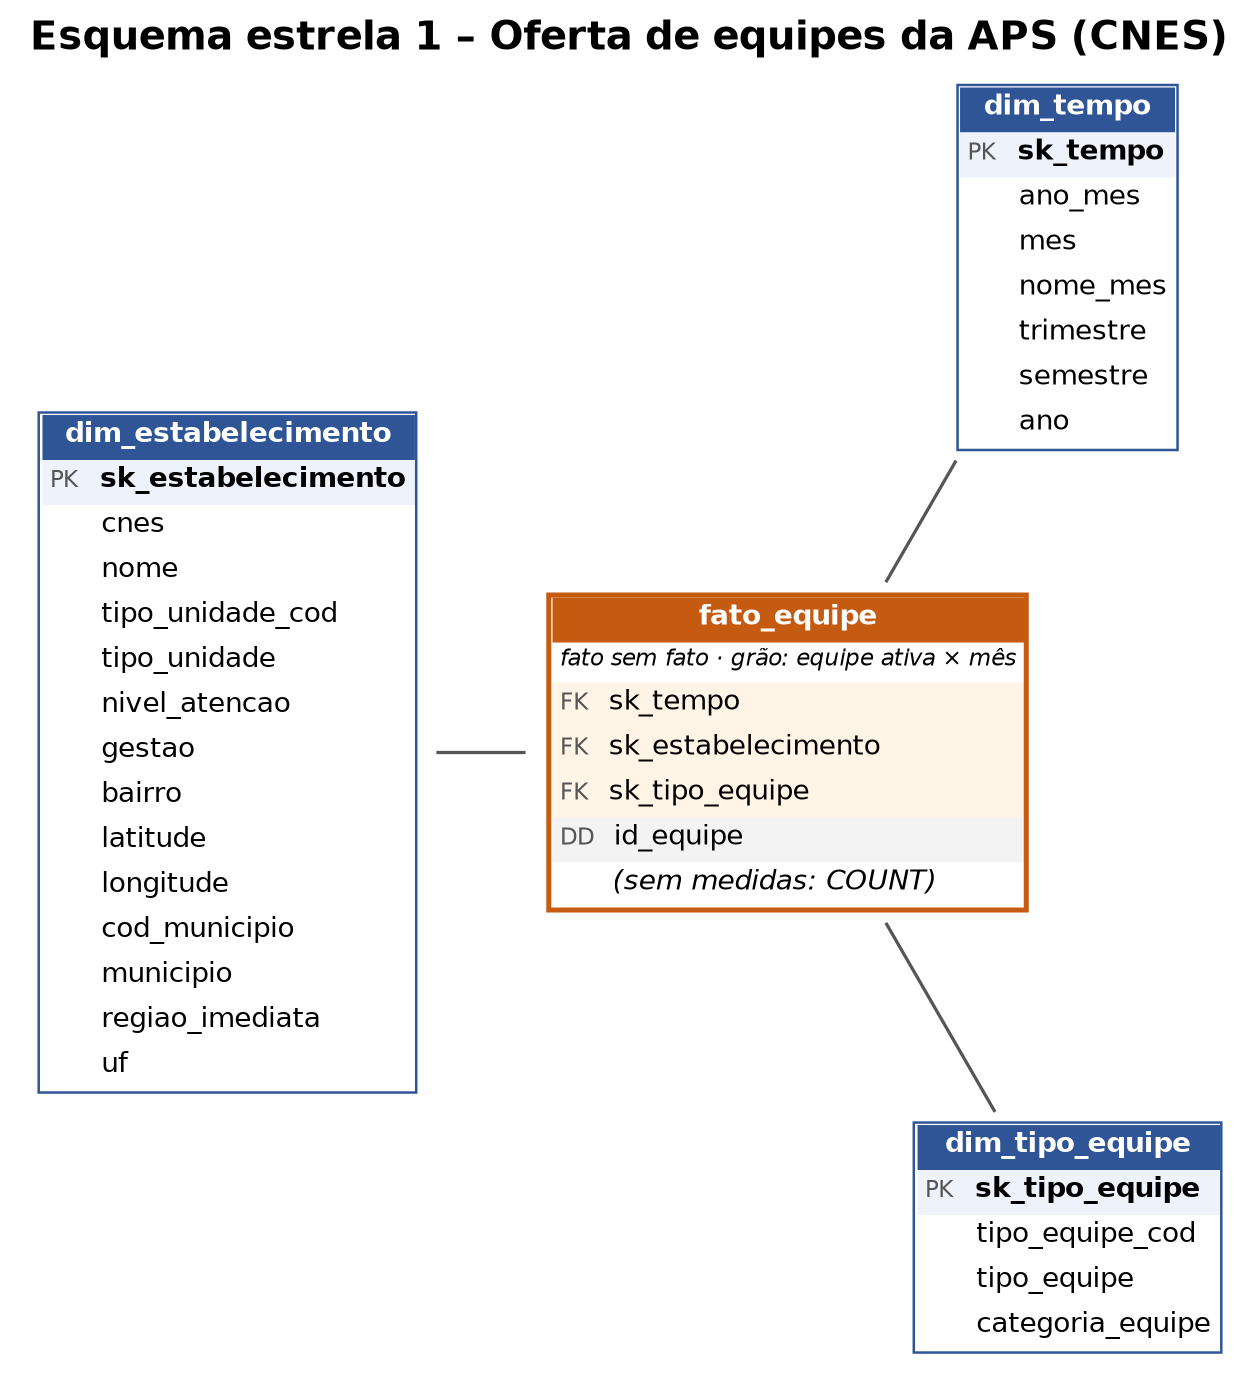
\includegraphics[width=\linewidth,height={19.5cm},keepaspectratio]{figuras/estrela_1_equipe.png}
\legenda{Figura 1 – Esquema estrela da oferta de equipes da atenção básica.}
\end{figure}

\subsubsection*{Hierarquias das dimensões}

\textbf{dim\_\allowbreak{}tempo}\par\nopagebreak\smallskip

\begin{hierarquias}\texttt{ano\_\allowbreak{}mes ≤ trimestre ≤ semestre ≤ ano}\end{hierarquias}

\textbf{dim\_\allowbreak{}estabelecimento}\par\nopagebreak\smallskip

\begin{hierarquias}\texttt{cnes ≤ tipo\_\allowbreak{}unidade ≤ nivel\_\allowbreak{}atencao}\\\texttt{cnes ≤ bairro ≤ municipio ≤ regiao\_\allowbreak{}imediata ≤ uf}\end{hierarquias}

\textbf{dim\_\allowbreak{}tipo\_\allowbreak{}equipe}\par\nopagebreak\smallskip

\begin{hierarquias}\texttt{tipo\_\allowbreak{}equipe\_\allowbreak{}cod ≤ categoria\_\allowbreak{}equipe}\end{hierarquias}

\subsubsection*{Funções de agregação}

\par\noindent\begin{minipage}{\linewidth}\small\rowcolors{2}{white}{linhapar}\begin{tabular}{|>{\raggedright\arraybackslash}p{\dimexpr0.2822\linewidth-2\tabcolsep-1.33\arrayrulewidth\relax}|>{\raggedright\arraybackslash}p{\dimexpr0.2209\linewidth-2\tabcolsep-1.33\arrayrulewidth\relax}|>{\raggedright\arraybackslash}p{\dimexpr0.4969\linewidth-2\tabcolsep-1.33\arrayrulewidth\relax}|}\hline\rowcolor{azul}\color{white}\bfseries Fato & \color{white}\bfseries Tipo & \color{white}\bfseries Função de agregação \\ \hline
número de equipes (contagem de linhas) & Semiaditivo & CONTAGEM no mesmo mês; entre meses, MÉDIA das contagens mensais ou valor do ÚLTIMO mês \\ \hline\end{tabular}\end{minipage}\par\medskip

\FloatBarrier\subsection*{2.2 Esquema estrela 2 – Internações hospitalares}\addcontentsline{toc}{subsection}{2.2 Esquema estrela 2 – Internações hospitalares}

\begin{figure}[!htbp]\centering
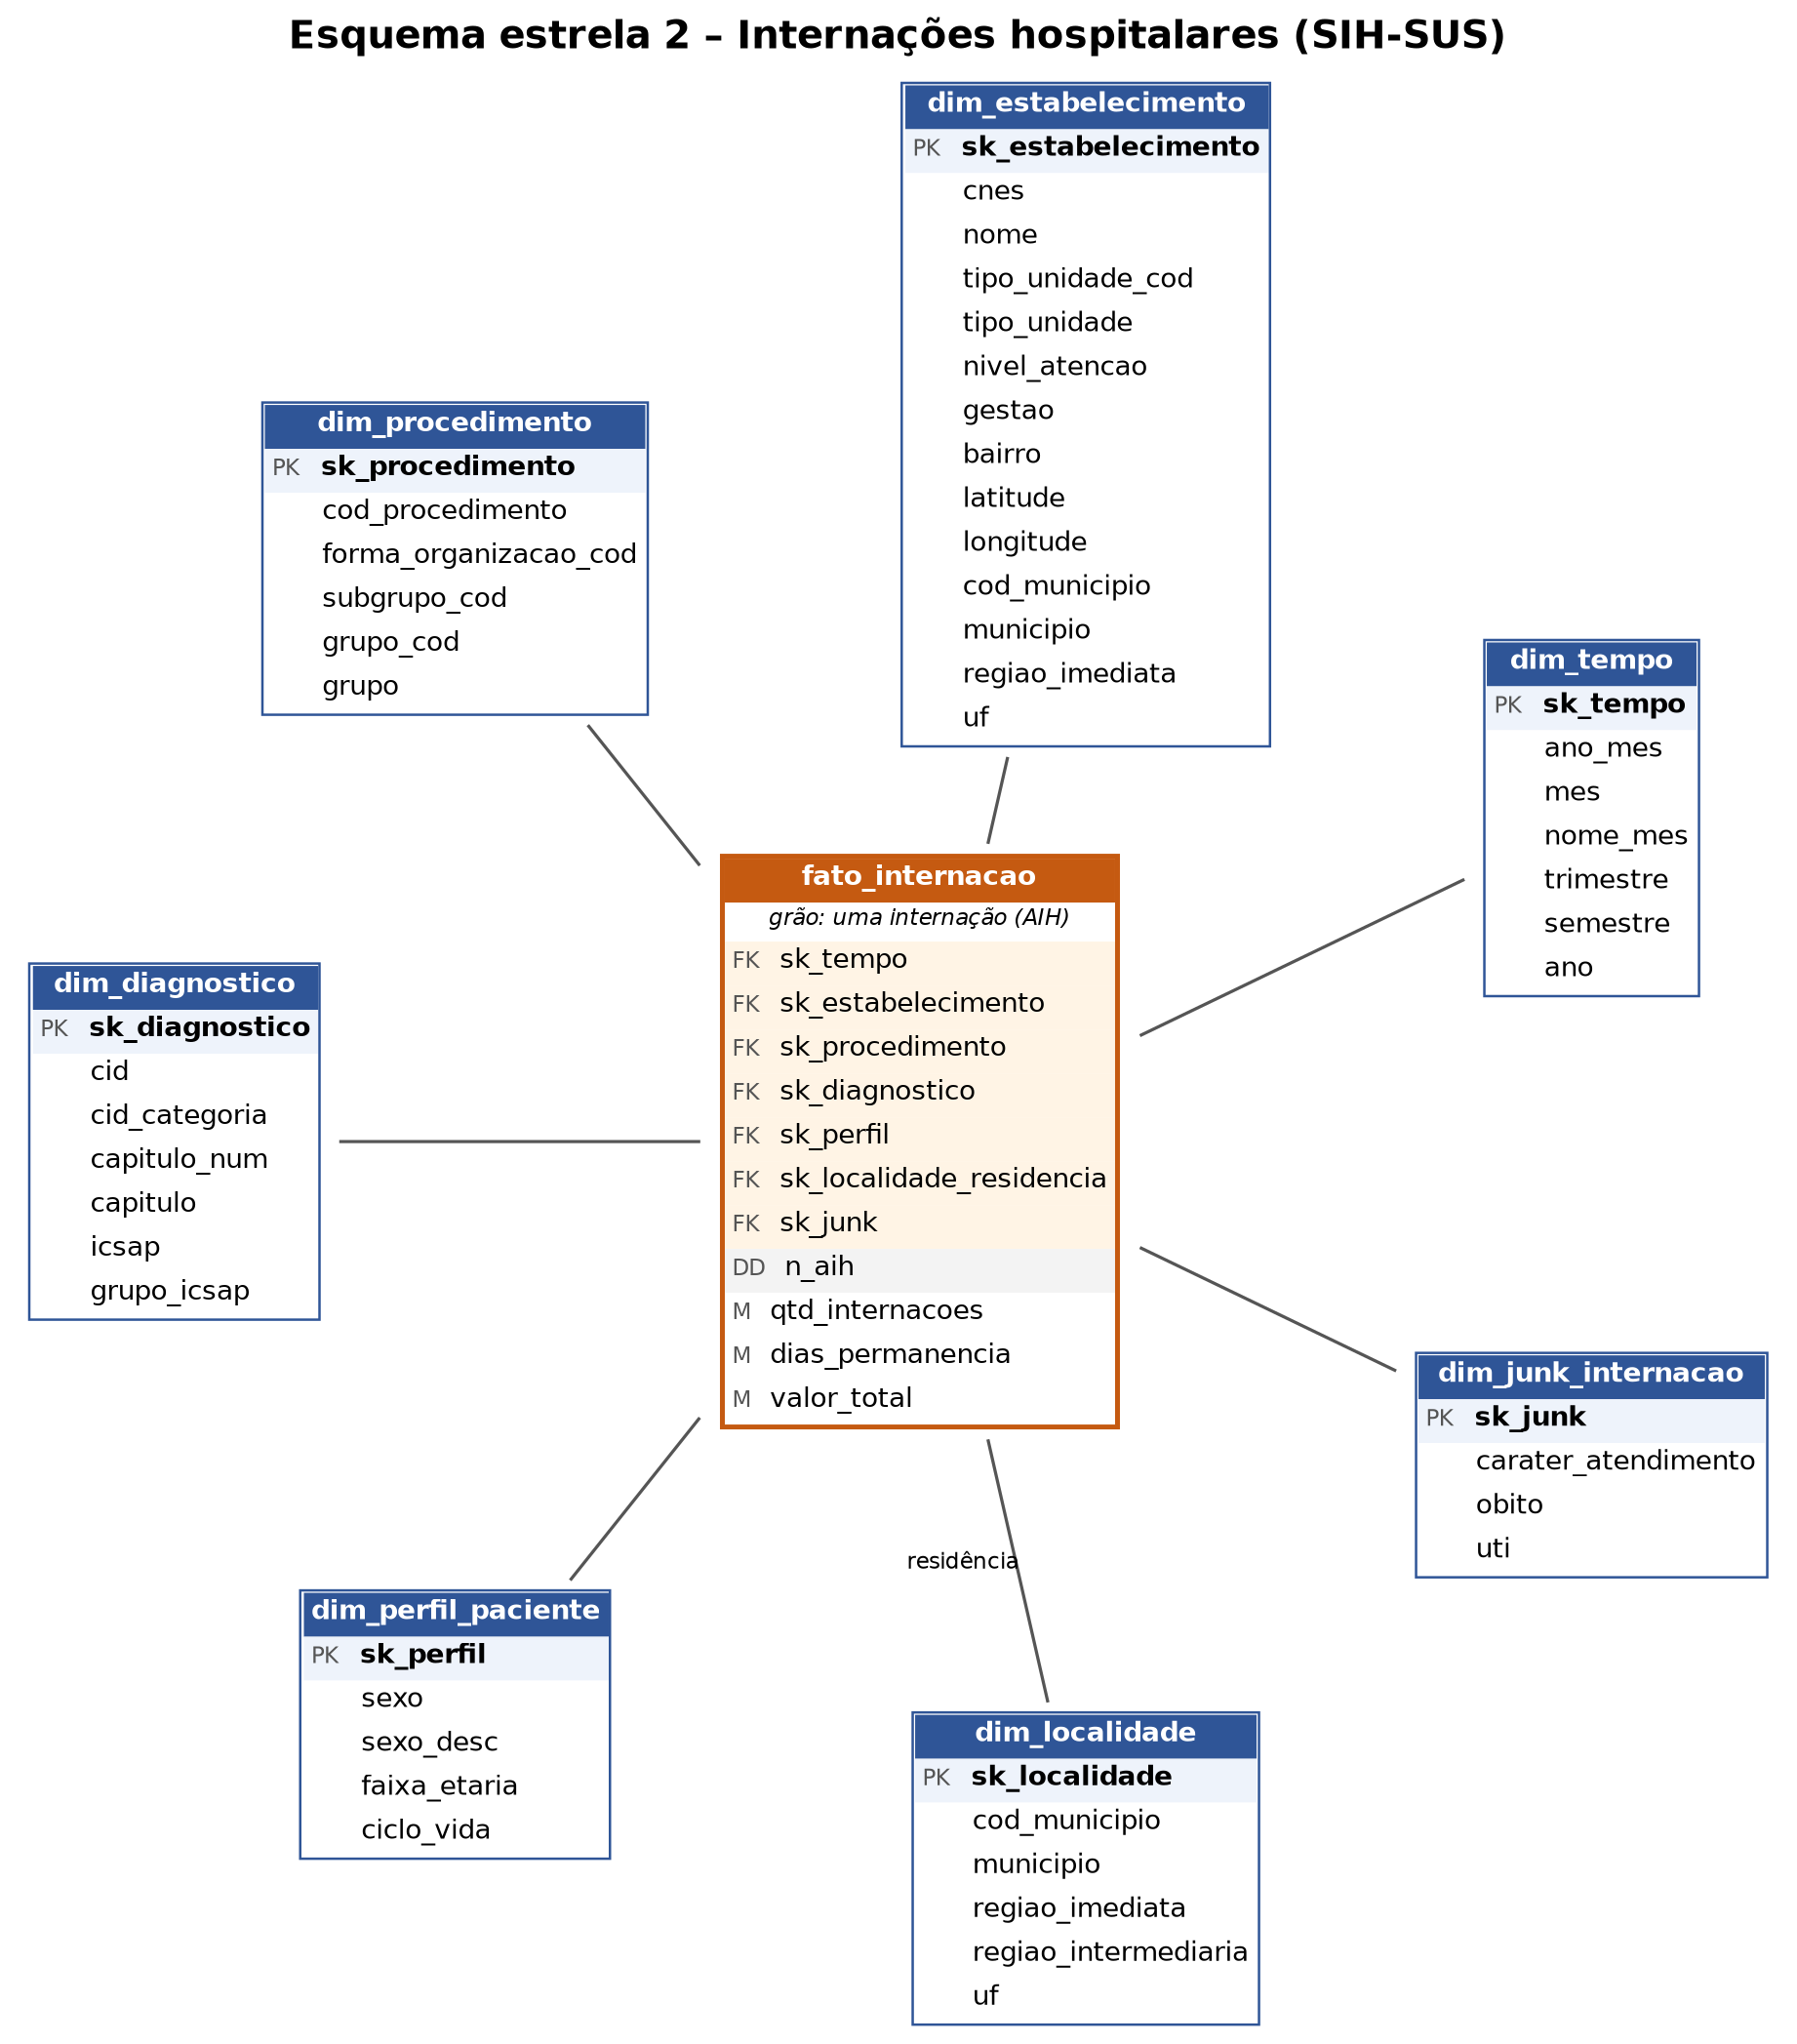
\includegraphics[width=\linewidth,height={19.5cm},keepaspectratio]{figuras/estrela_2_internacao.png}
\legenda{Figura 2 – Esquema estrela das internações hospitalares.}
\end{figure}

\subsubsection*{Hierarquias das dimensões}

\textbf{dim\_\allowbreak{}tempo}\par\nopagebreak\smallskip

\begin{hierarquias}\texttt{ano\_\allowbreak{}mes ≤ trimestre ≤ semestre ≤ ano}\end{hierarquias}

\textbf{dim\_\allowbreak{}estabelecimento}\par\nopagebreak\smallskip

\begin{hierarquias}\texttt{cnes ≤ tipo\_\allowbreak{}unidade ≤ nivel\_\allowbreak{}atencao}\\\texttt{cnes ≤ bairro ≤ municipio ≤ regiao\_\allowbreak{}imediata ≤ uf}\end{hierarquias}

\textbf{dim\_\allowbreak{}procedimento}\par\nopagebreak\smallskip

\begin{hierarquias}\texttt{cod\_\allowbreak{}procedimento ≤ forma\_\allowbreak{}organizacao\_\allowbreak{}cod ≤ subgrupo\_\allowbreak{}cod ≤ grupo\_\allowbreak{}cod}\end{hierarquias}

\textbf{dim\_\allowbreak{}diagnostico}\par\nopagebreak\smallskip

\begin{hierarquias}\texttt{cid ≤ cid\_\allowbreak{}categoria ≤ capitulo}\\\texttt{cid ≤ grupo\_\allowbreak{}icsap ≤ icsap}\end{hierarquias}

\textbf{dim\_\allowbreak{}perfil\_\allowbreak{}paciente}\par\nopagebreak\smallskip

\begin{hierarquias}\texttt{faixa\_\allowbreak{}etaria ≤ ciclo\_\allowbreak{}vida}\\\texttt{(sexo é descritivo, sem hierarquia)}\end{hierarquias}

\textbf{dim\_\allowbreak{}localidade}\par\nopagebreak\smallskip

\begin{hierarquias}\texttt{municipio ≤ regiao\_\allowbreak{}imediata ≤ regiao\_\allowbreak{}intermediaria ≤ uf}\end{hierarquias}

\textbf{dim\_\allowbreak{}junk\_\allowbreak{}internacao}\par\nopagebreak\smallskip

\begin{hierarquias}\texttt{(sem hierarquia; atributos descritivos)}\end{hierarquias}

\subsubsection*{Funções de agregação}

\par\noindent\begin{minipage}{\linewidth}\small\rowcolors{2}{white}{linhapar}\begin{tabular}{|>{\raggedright\arraybackslash}p{\dimexpr0.2822\linewidth-2\tabcolsep-1.33\arrayrulewidth\relax}|>{\raggedright\arraybackslash}p{\dimexpr0.2209\linewidth-2\tabcolsep-1.33\arrayrulewidth\relax}|>{\raggedright\arraybackslash}p{\dimexpr0.4969\linewidth-2\tabcolsep-1.33\arrayrulewidth\relax}|}\hline\rowcolor{azul}\color{white}\bfseries Fato & \color{white}\bfseries Tipo & \color{white}\bfseries Função de agregação \\ \hline
qtd\_\allowbreak{}internacoes & Aditivo & SOMA \\ \hline
dias\_\allowbreak{}permanencia & Aditivo & SOMA \\ \hline
valor\_\allowbreak{}total & Aditivo & SOMA \\ \hline
média de permanência (derivado) & Não aditivo & SOMA(dias\_\allowbreak{}permanencia) ÷ SOMA(qtd\_\allowbreak{}internacoes) \\ \hline
taxa de ICSAP (derivado) & Não aditivo & SOMA(qtd\_\allowbreak{}internacoes ICSAP) ÷ população × 10.000 \\ \hline\end{tabular}\end{minipage}\par\medskip

\FloatBarrier\subsection*{2.3 Esquema estrela 3 – Produção ambulatorial}\addcontentsline{toc}{subsection}{2.3 Esquema estrela 3 – Produção ambulatorial}

\begin{figure}[!htbp]\centering
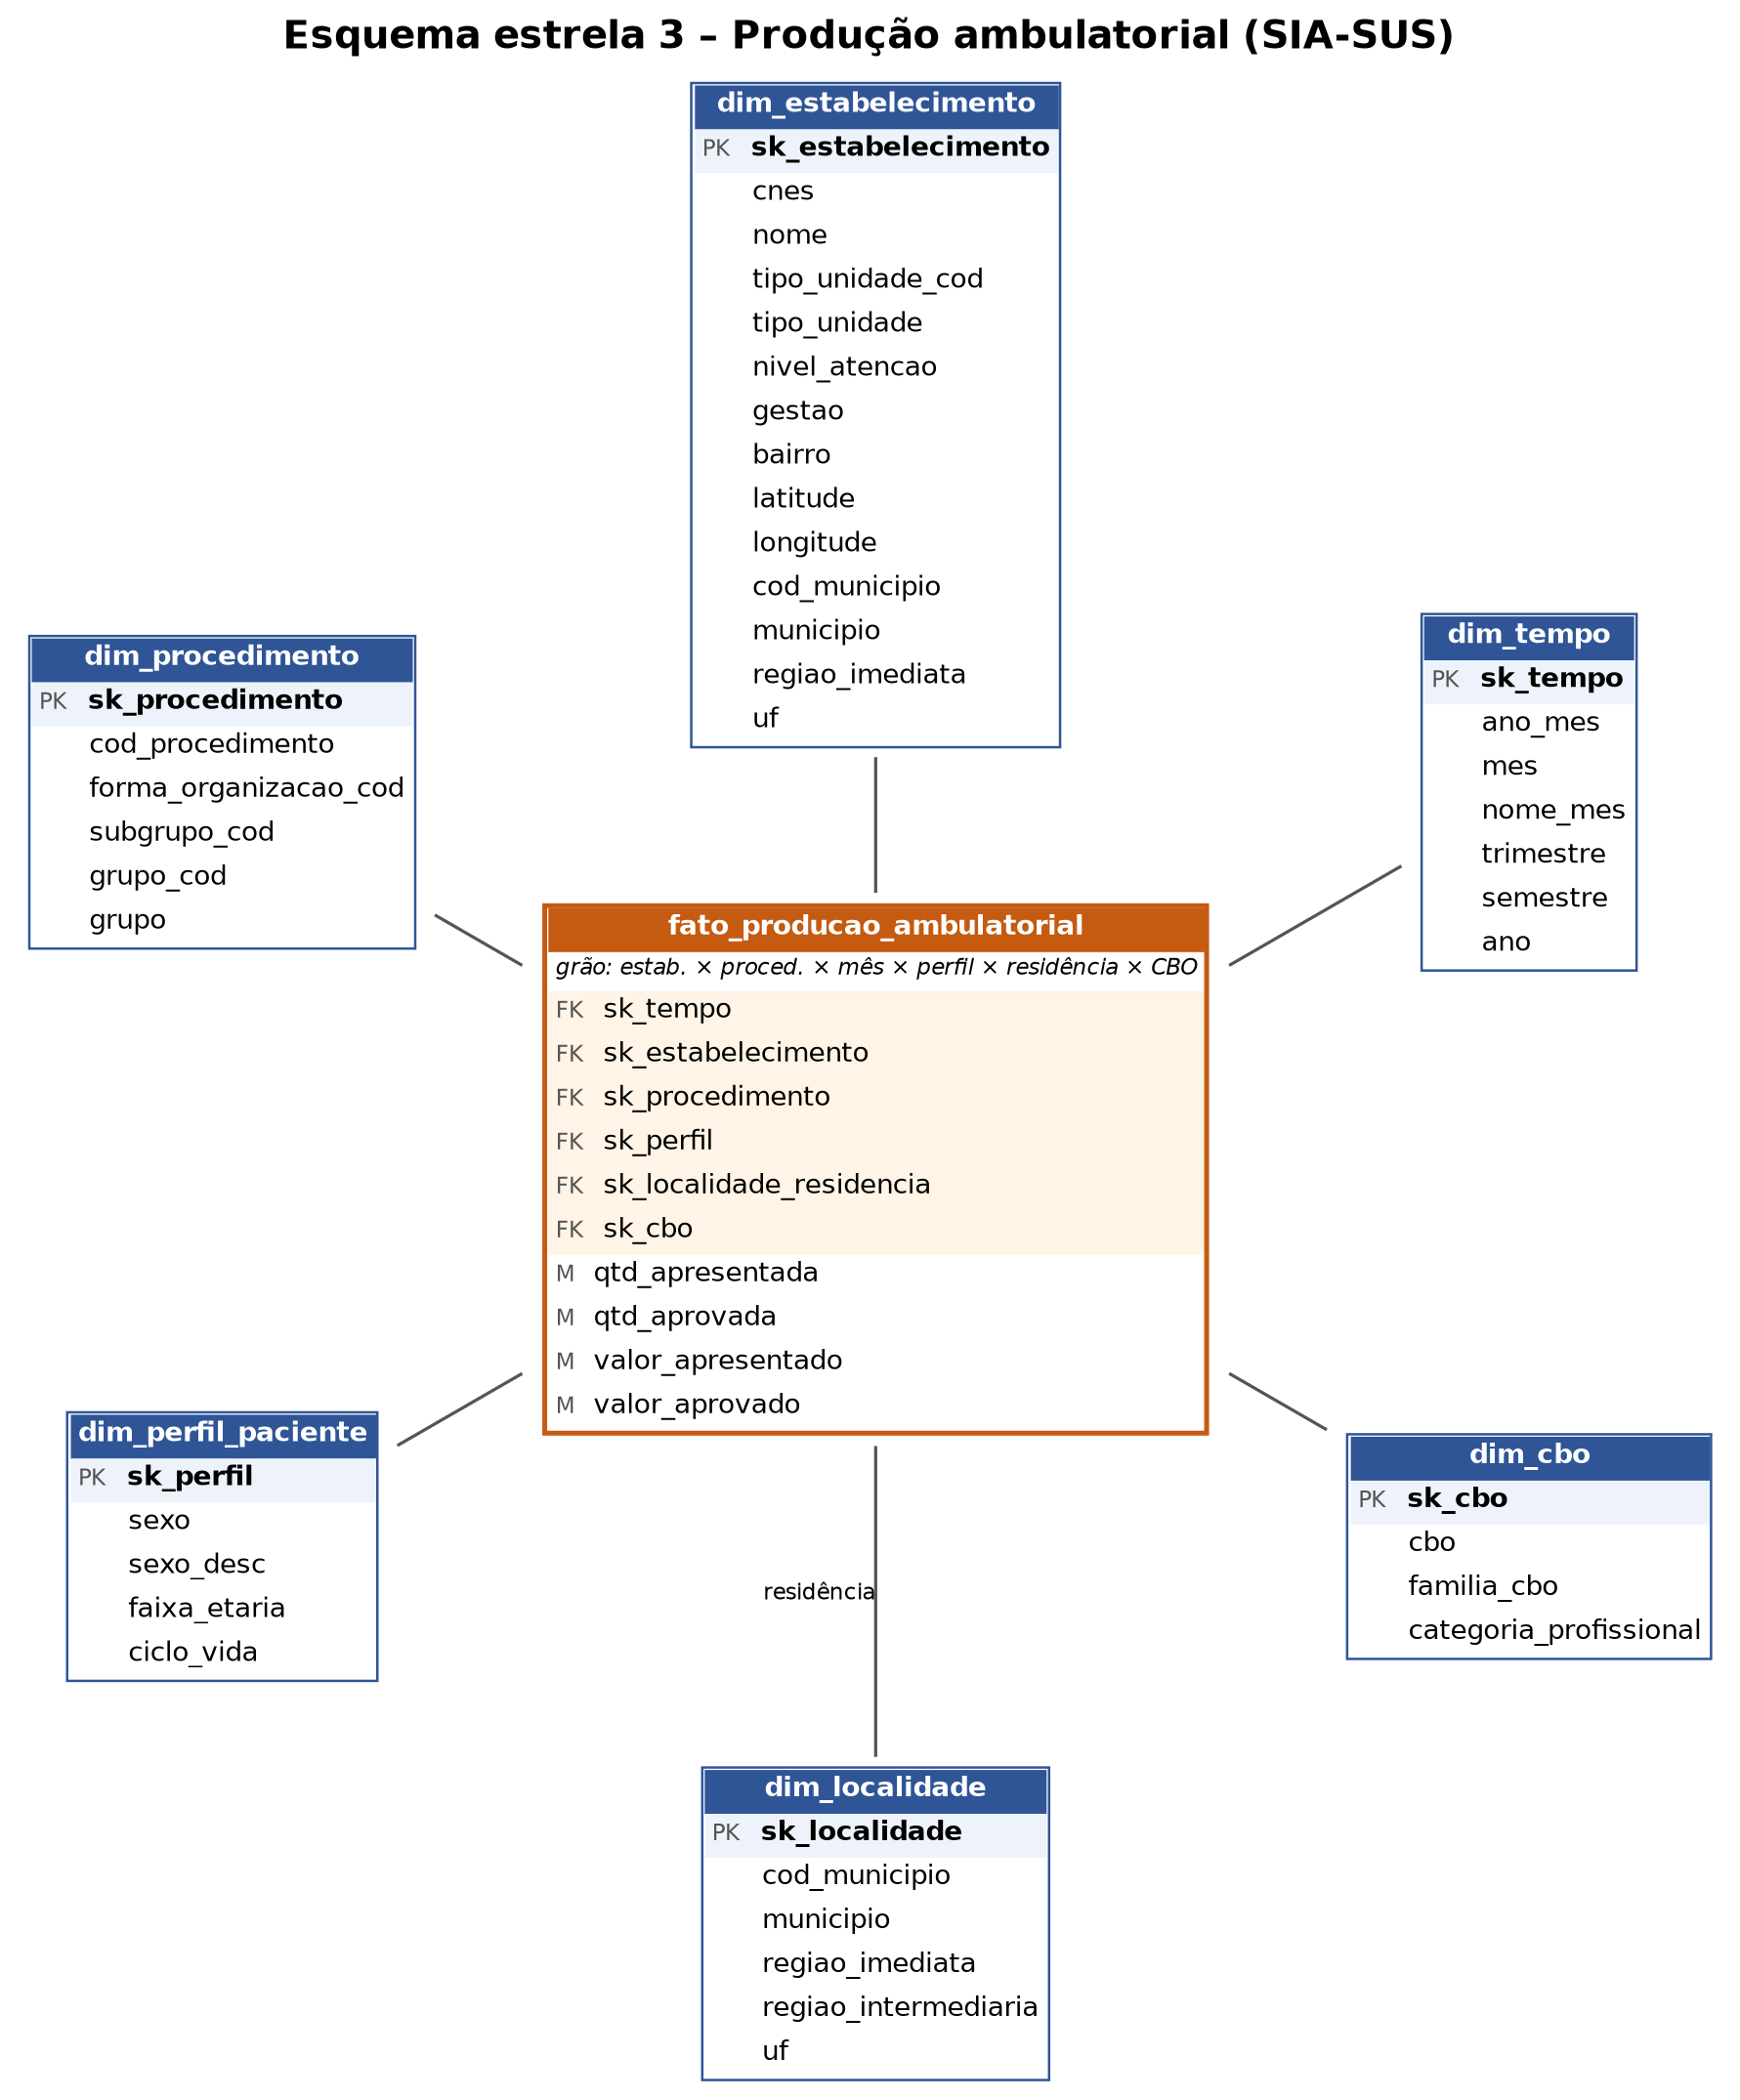
\includegraphics[width=\linewidth,height={19.5cm},keepaspectratio]{figuras/estrela_3_producao.png}
\legenda{Figura 3 – Esquema estrela da produção ambulatorial.}
\end{figure}

\subsubsection*{Hierarquias das dimensões}

\textbf{dim\_\allowbreak{}tempo}\par\nopagebreak\smallskip

\begin{hierarquias}\texttt{ano\_\allowbreak{}mes ≤ trimestre ≤ semestre ≤ ano}\end{hierarquias}

\textbf{dim\_\allowbreak{}estabelecimento}\par\nopagebreak\smallskip

\begin{hierarquias}\texttt{cnes ≤ tipo\_\allowbreak{}unidade ≤ nivel\_\allowbreak{}atencao}\\\texttt{cnes ≤ bairro ≤ municipio ≤ regiao\_\allowbreak{}imediata ≤ uf}\end{hierarquias}

\textbf{dim\_\allowbreak{}procedimento}\par\nopagebreak\smallskip

\begin{hierarquias}\texttt{cod\_\allowbreak{}procedimento ≤ forma\_\allowbreak{}organizacao\_\allowbreak{}cod ≤ subgrupo\_\allowbreak{}cod ≤ grupo\_\allowbreak{}cod}\end{hierarquias}

\textbf{dim\_\allowbreak{}perfil\_\allowbreak{}paciente}\par\nopagebreak\smallskip

\begin{hierarquias}\texttt{faixa\_\allowbreak{}etaria ≤ ciclo\_\allowbreak{}vida}\\\texttt{(sexo é descritivo, sem hierarquia)}\end{hierarquias}

\textbf{dim\_\allowbreak{}localidade}\par\nopagebreak\smallskip

\begin{hierarquias}\texttt{municipio ≤ regiao\_\allowbreak{}imediata ≤ regiao\_\allowbreak{}intermediaria ≤ uf}\end{hierarquias}

\textbf{dim\_\allowbreak{}cbo}\par\nopagebreak\smallskip

\begin{hierarquias}\texttt{cbo ≤ familia\_\allowbreak{}cbo ≤ categoria\_\allowbreak{}profissional}\end{hierarquias}

\subsubsection*{Funções de agregação}

\par\noindent\begin{minipage}{\linewidth}\small\rowcolors{2}{white}{linhapar}\begin{tabular}{|>{\raggedright\arraybackslash}p{\dimexpr0.2822\linewidth-2\tabcolsep-1.33\arrayrulewidth\relax}|>{\raggedright\arraybackslash}p{\dimexpr0.2209\linewidth-2\tabcolsep-1.33\arrayrulewidth\relax}|>{\raggedright\arraybackslash}p{\dimexpr0.4969\linewidth-2\tabcolsep-1.33\arrayrulewidth\relax}|}\hline\rowcolor{azul}\color{white}\bfseries Fato & \color{white}\bfseries Tipo & \color{white}\bfseries Função de agregação \\ \hline
qtd\_\allowbreak{}apresentada & Aditivo & SOMA \\ \hline
qtd\_\allowbreak{}aprovada & Aditivo & SOMA \\ \hline
valor\_\allowbreak{}apresentado & Aditivo & SOMA \\ \hline
valor\_\allowbreak{}aprovado & Aditivo & SOMA \\ \hline
taxa de aprovação (derivado) & Não aditivo & SOMA(qtd\_\allowbreak{}aprovada) ÷ SOMA(qtd\_\allowbreak{}apresentada) \\ \hline\end{tabular}\end{minipage}\par\medskip

\FloatBarrier\subsection*{2.4 Aspectos adicionais de modelagem}\addcontentsline{toc}{subsection}{2.4 Aspectos adicionais de modelagem}

\begin{itemize}\item \textbf{Chaves artificiais:} todas as dimensões têm chave primária artificial, o que isola o DW de mudanças nos códigos das fontes, permite o membro “Não informado” (chave 0) e reduz o tamanho das tabelas de fatos.
\item \textbf{Tabela bugiganga:} \texttt{dim\_\allowbreak{}junk\_\allowbreak{}internacao} reúne caráter do atendimento, óbito e uso de UTI.
\item \textbf{Dimensões degeneradas:} \texttt{n\_\allowbreak{}aih} em fato\_\allowbreak{}internacao e \texttt{id\_\allowbreak{}equipe} em fato\_\allowbreak{}equipe. São identificadores sem outros atributos, úteis para contar itens distintos e rastrear o registro na fonte.
\item \textbf{Tabela de fatos sem fato:} \texttt{fato\_\allowbreak{}equipe} registra apenas a existência de uma equipe ativa em um estabelecimento em um mês; a análise é feita por contagem.
\item \textbf{Mini-dimensão:} \texttt{dim\_\allowbreak{}perfil\_\allowbreak{}paciente} separa os atributos demográficos do paciente, que no SUS não tem identificação pública, em uma dimensão pequena e compartilhada.\end{itemize}

\clearpage

\FloatBarrier\subsection*{2.5 Constelação de fatos}\addcontentsline{toc}{subsection}{2.5 Constelação de fatos}

\begin{figure}[!htbp]\centering
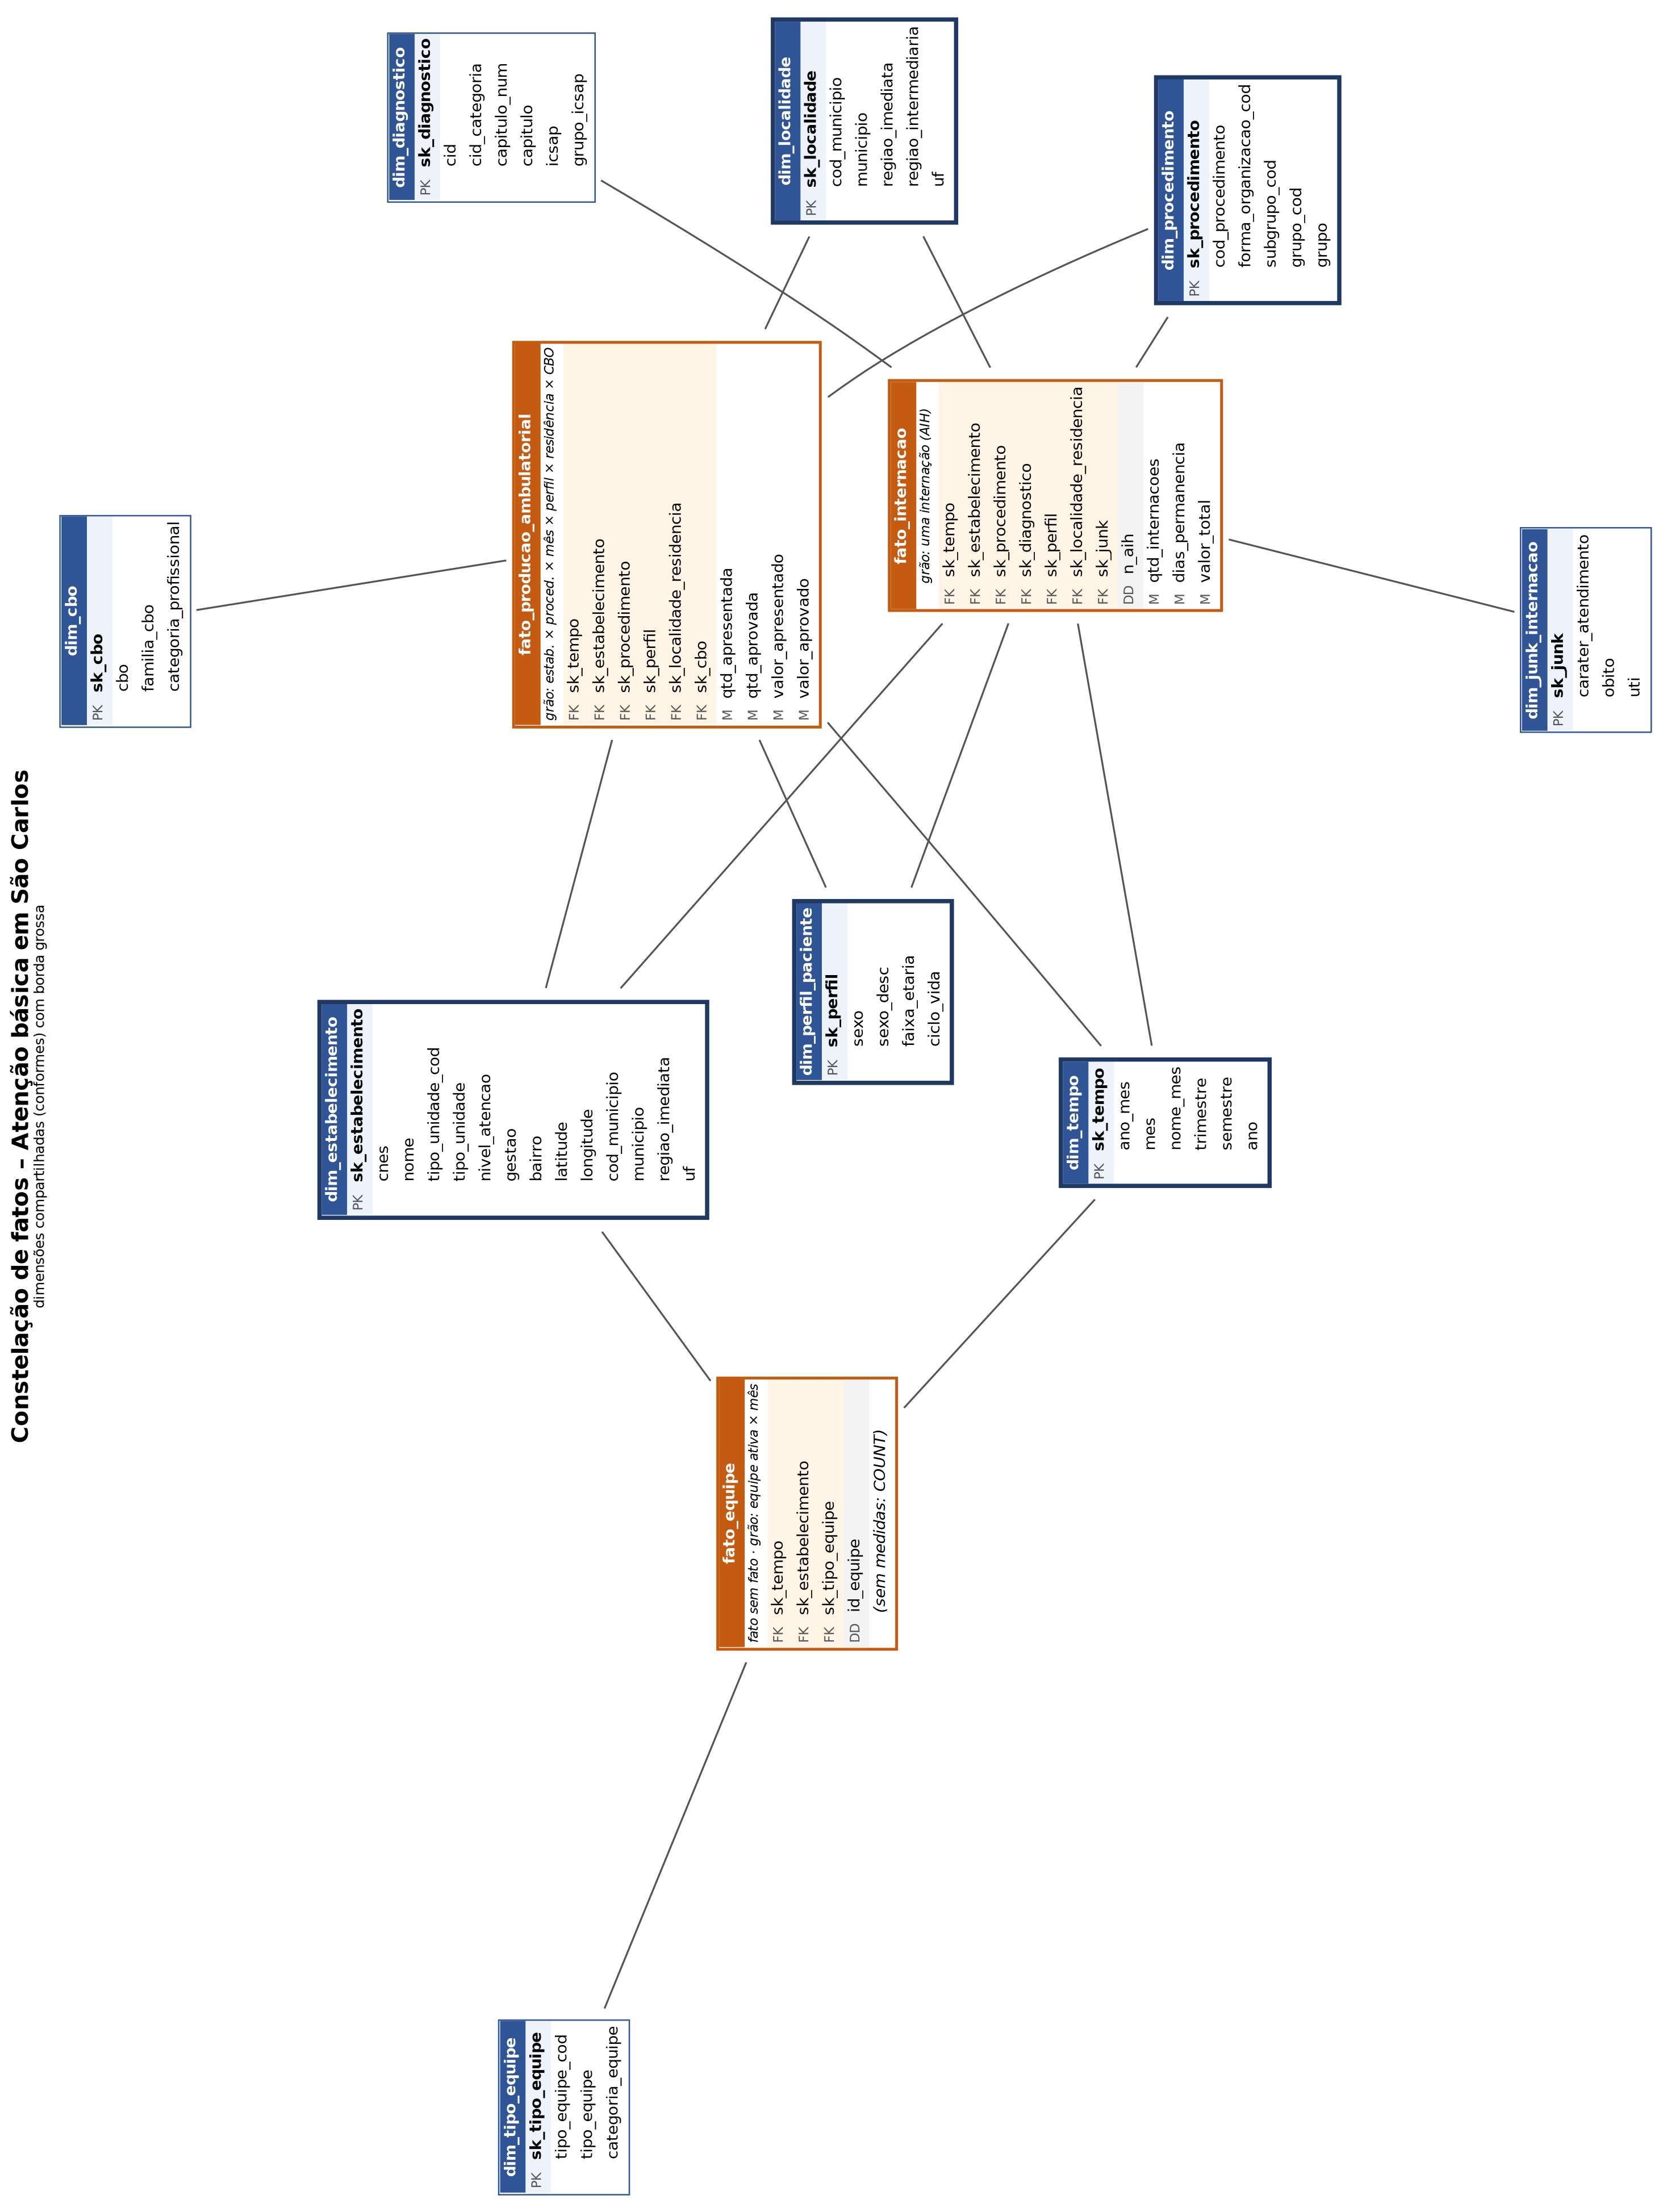
\includegraphics[width=\linewidth,height={20.5cm},keepaspectratio]{figuras/constelacao_rot.png}
\legenda{Figura 4 – Constelação de fatos (imagem girada). Dimensões compartilhadas com borda grossa.}
\end{figure}

\subsubsection*{Processo de projeto da constelação}

A constelação foi obtida em quatro passos:


\begin{itemize}\item \textbf{1. Modelagem independente.} Cada processo de negócio foi modelado como uma estrela própria, com seu grão, suas dimensões e seus fatos (Figuras 1 a 3).
\item \textbf{2. Identificação das dimensões em comum.} Comparando as estrelas, identificaram-se as dimensões que aparecem em mais de uma: tempo, estabelecimento, procedimento, perfil do paciente e localidade.
\item \textbf{3. Conformação das dimensões.} Cada dimensão comum passou a ter uma única definição, com a mesma chave, os mesmos atributos e os mesmos valores em todas as estrelas. Por exemplo, o tempo usa sempre o mês de competência, o sexo usa sempre M/F/I e o estabelecimento usa sempre o CNES com 7 dígitos, qualquer que seja a fonte. Foi para isso que o grão do tempo foi fixado no mês, o menor nível comum às três fontes.
\item \textbf{4. Junção.} As três tabelas de fatos passam a apontar para as mesmas tabelas de dimensão, formando a constelação. Isso permite comparar os três processos na mesma análise por meio da operação drill-across (Consulta 5).\end{itemize}

A matriz abaixo resume quais dimensões são usadas por cada tabela de fatos.


\par\noindent\begin{minipage}{\linewidth}\small\rowcolors{2}{white}{linhapar}\begin{tabular}{|>{\raggedright\arraybackslash}p{\dimexpr0.3067\linewidth-2\tabcolsep-1.25\arrayrulewidth\relax}|>{\raggedright\arraybackslash}p{\dimexpr0.2025\linewidth-2\tabcolsep-1.25\arrayrulewidth\relax}|>{\raggedright\arraybackslash}p{\dimexpr0.2147\linewidth-2\tabcolsep-1.25\arrayrulewidth\relax}|>{\raggedright\arraybackslash}p{\dimexpr0.2761\linewidth-2\tabcolsep-1.25\arrayrulewidth\relax}|}\hline\rowcolor{azul}\color{white}\bfseries Dimensão & \color{white}\bfseries fato\_\allowbreak{}equipe & \color{white}\bfseries fato\_\allowbreak{}internacao & \color{white}\bfseries fato\_\allowbreak{}producao\_\allowbreak{}ambulatorial \\ \hline
dim\_\allowbreak{}tempo & ✓ & ✓ & ✓ \\ \hline
dim\_\allowbreak{}estabelecimento & ✓ & ✓ & ✓ \\ \hline
dim\_\allowbreak{}procedimento &  & ✓ & ✓ \\ \hline
dim\_\allowbreak{}perfil\_\allowbreak{}paciente &  & ✓ & ✓ \\ \hline
dim\_\allowbreak{}localidade &  & ✓ & ✓ \\ \hline
dim\_\allowbreak{}tipo\_\allowbreak{}equipe & ✓ &  &  \\ \hline
dim\_\allowbreak{}diagnostico &  & ✓ &  \\ \hline
dim\_\allowbreak{}junk\_\allowbreak{}internacao &  & ✓ &  \\ \hline
dim\_\allowbreak{}cbo &  &  & ✓ \\ \hline\end{tabular}\end{minipage}\par\medskip

\clearpage

\FloatBarrier\section*{3. Consultas}\addcontentsline{toc}{section}{3. Consultas}

As consultas abaixo são as principais perguntas que o data warehouse deve responder. Todas usam como filtro o município de São Carlos, pela residência do paciente (demanda) ou pela localização do estabelecimento (oferta).


Todas foram executadas no DW povoado com os dados reais de 2023 e 2024. Para cada uma, o relatório mostra o resultado obtido e uma captura da célula do notebook com o código SQL e a saída. Tabelas longas aparecem com início e fim, separados por “…”.


\FloatBarrier\subsection*{Consulta 1 – Roll-up}\addcontentsline{toc}{subsection}{Consulta 1 – Roll-up}

\begin{figure}[!htbp]\centering
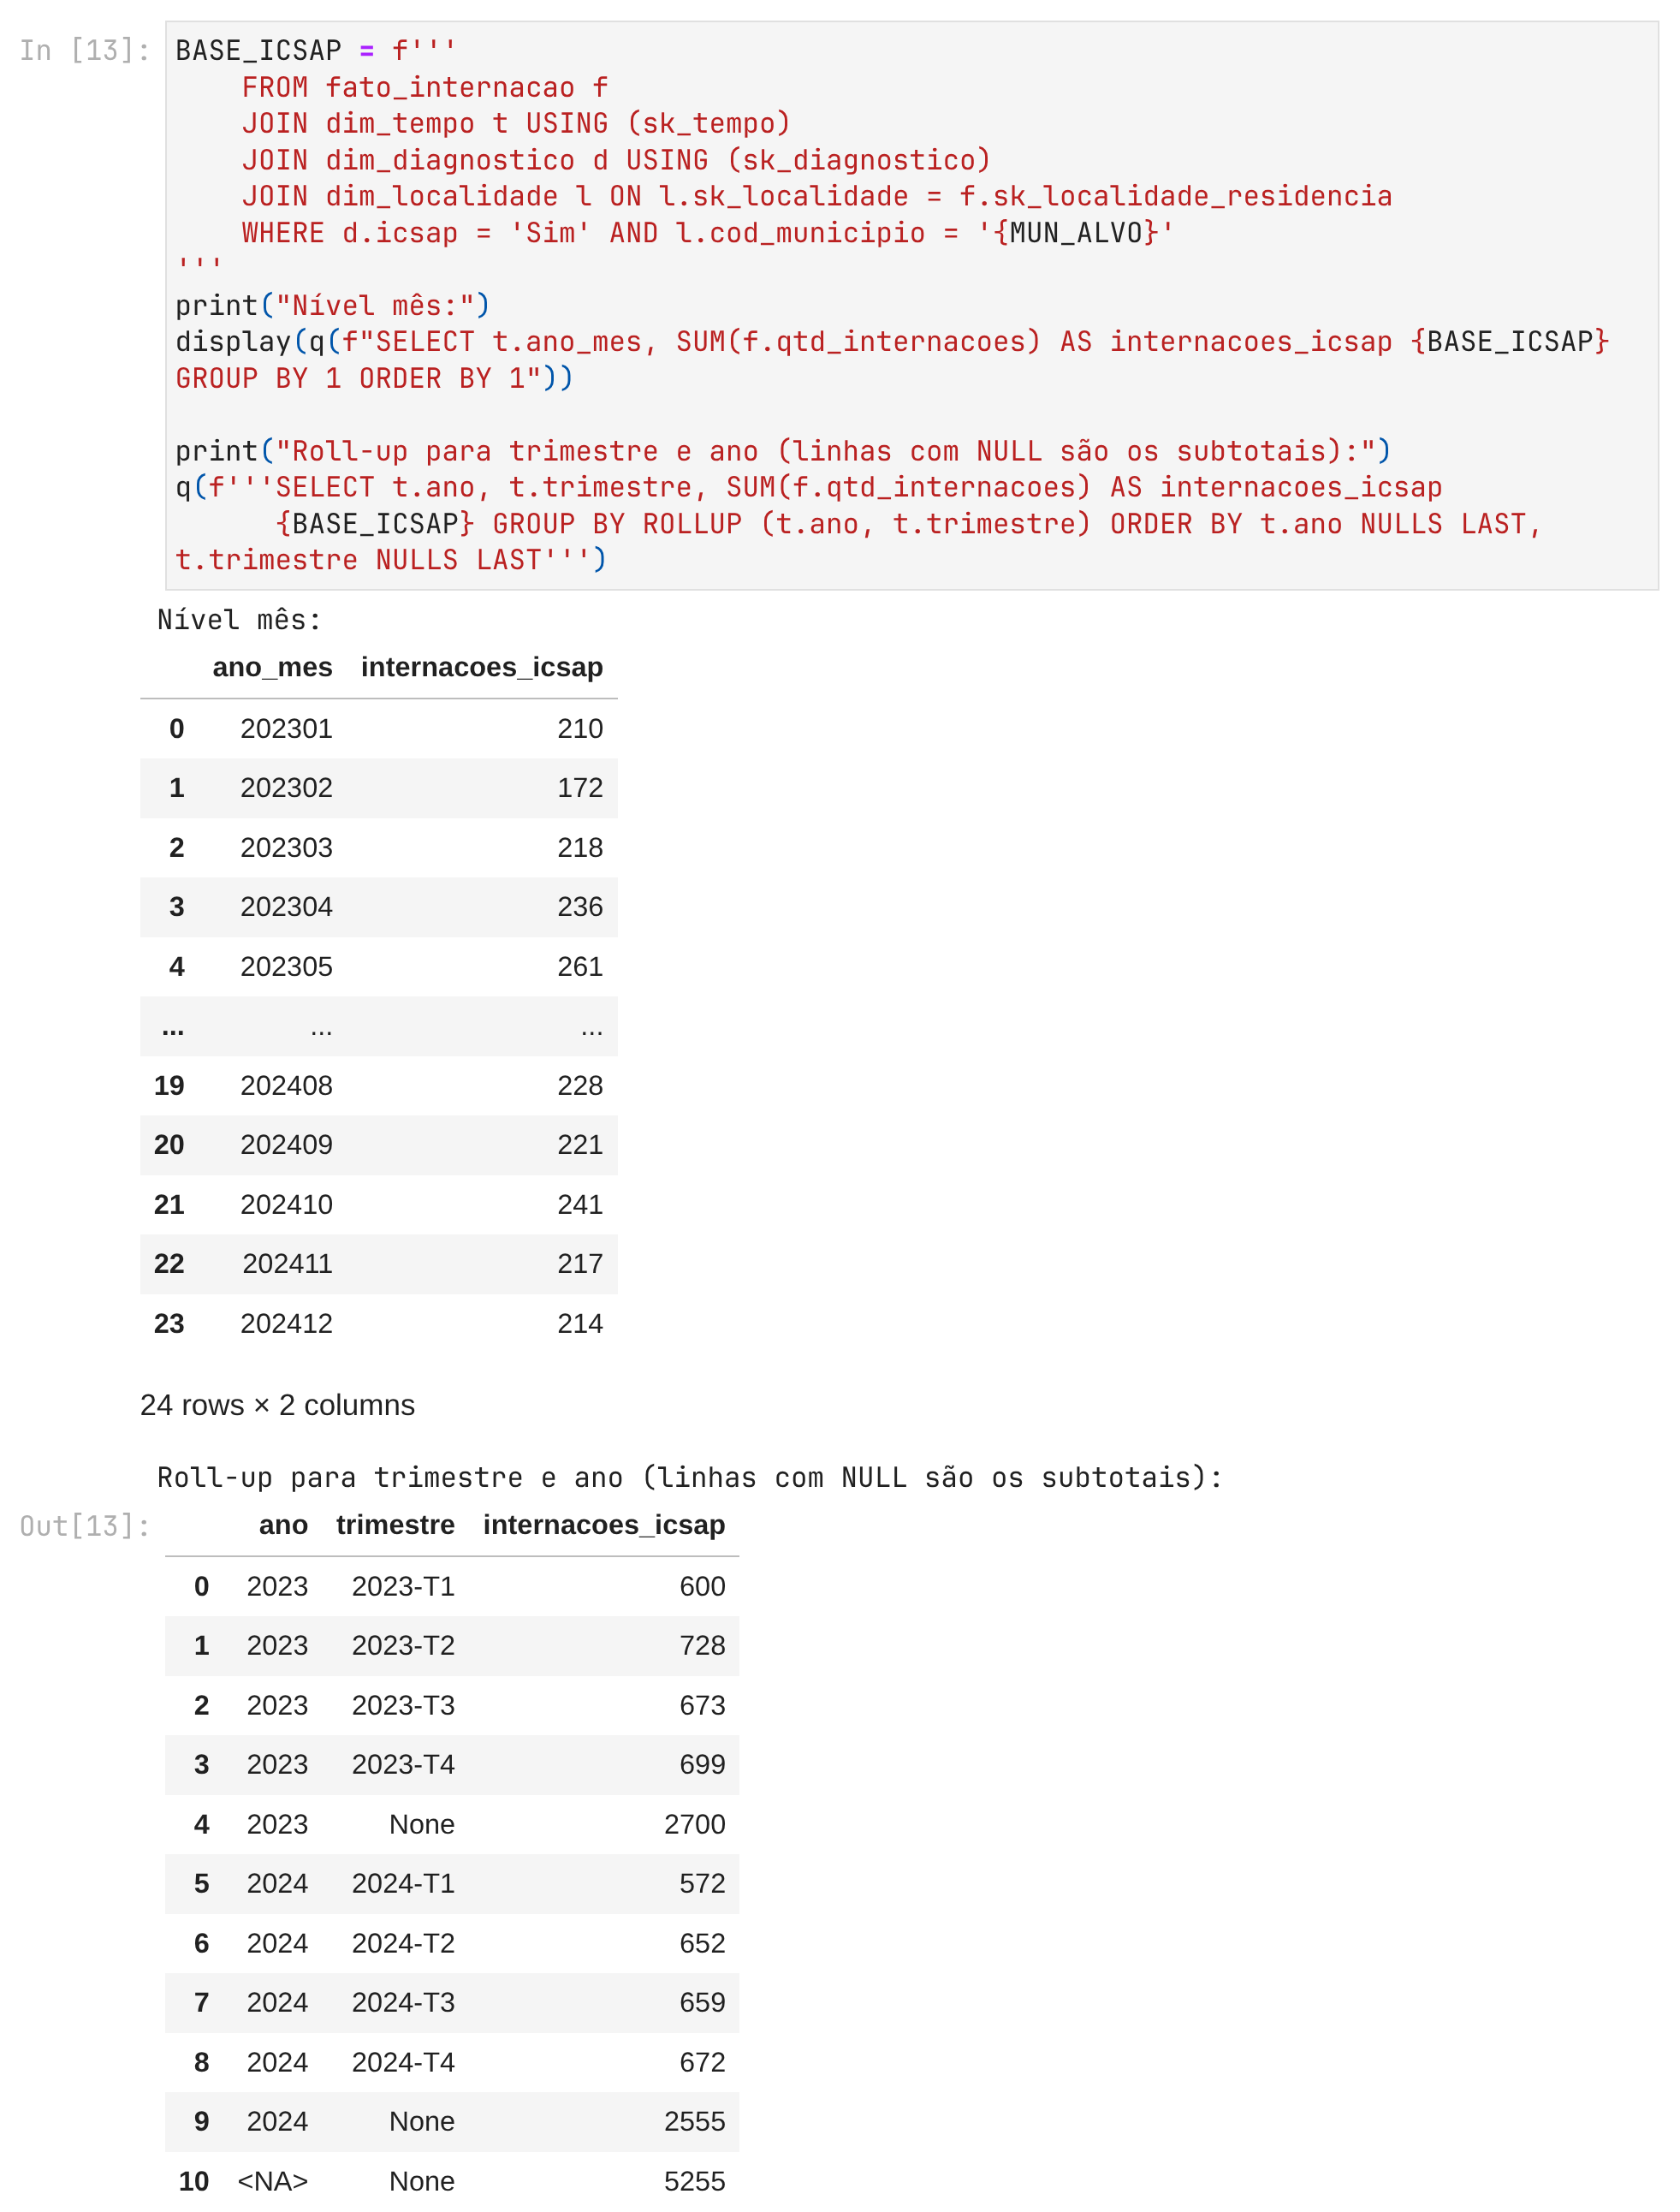
\includegraphics[width=\linewidth,height={\dimexpr\textheight-4\baselineskip\relax},keepaspectratio]{figuras/consulta1.png}
\legenda{Figura 5 – Consulta 1 no notebook: ICSAP por mês e roll-up para trimestre e ano (linhas com NULL são os subtotais).}
\end{figure}

\textbf{Operação OLAP:} Roll-up na dimensão tempo (ano\_\allowbreak{}mes → trimestre → ano).


\textbf{Consulta:} Qual o número de internações por condições sensíveis à atenção primária de residentes em São Carlos em cada mês? Em seguida, agregar o resultado por trimestre e por ano.


\textbf{Elementos do esquema:} Tabela de fatos: fato\_\allowbreak{}internacao. Dimensões: tempo (ano\_\allowbreak{}mes, trimestre, ano), diagnóstico (icsap = Sim), localidade (município de residência = São Carlos). Medida: SOMA de qtd\_\allowbreak{}internacoes.


\textbf{Importância e justificativa:} É o indicador central de efetividade da atenção básica. A visão mensal mostra sazonalidade (por exemplo, doenças respiratórias no inverno) e a visão anual mostra a tendência que interessa ao planejamento plurianual do município.


\textbf{Resultado com os dados reais:} Foram 5.255 internações por condições sensíveis à atenção primária de residentes nos dois anos, 16\% das 32.799 internações de residentes. No nível mês, o maior valor é dezembro de 2023 (291) e o menor, janeiro de 2024 (167); como o mês é o de processamento da AIH, parte dessa oscilação reflete o ritmo de apresentação dos hospitais. Subindo para trimestre, a série fica entre 572 e 728, e no ano passa de 2.700 (2023) para 2.555 (2024), queda de cerca de 5\%.


\FloatBarrier\subsection*{Consulta 2 – Drill-down}\addcontentsline{toc}{subsection}{Consulta 2 – Drill-down}

\begin{figure}[!htbp]\centering
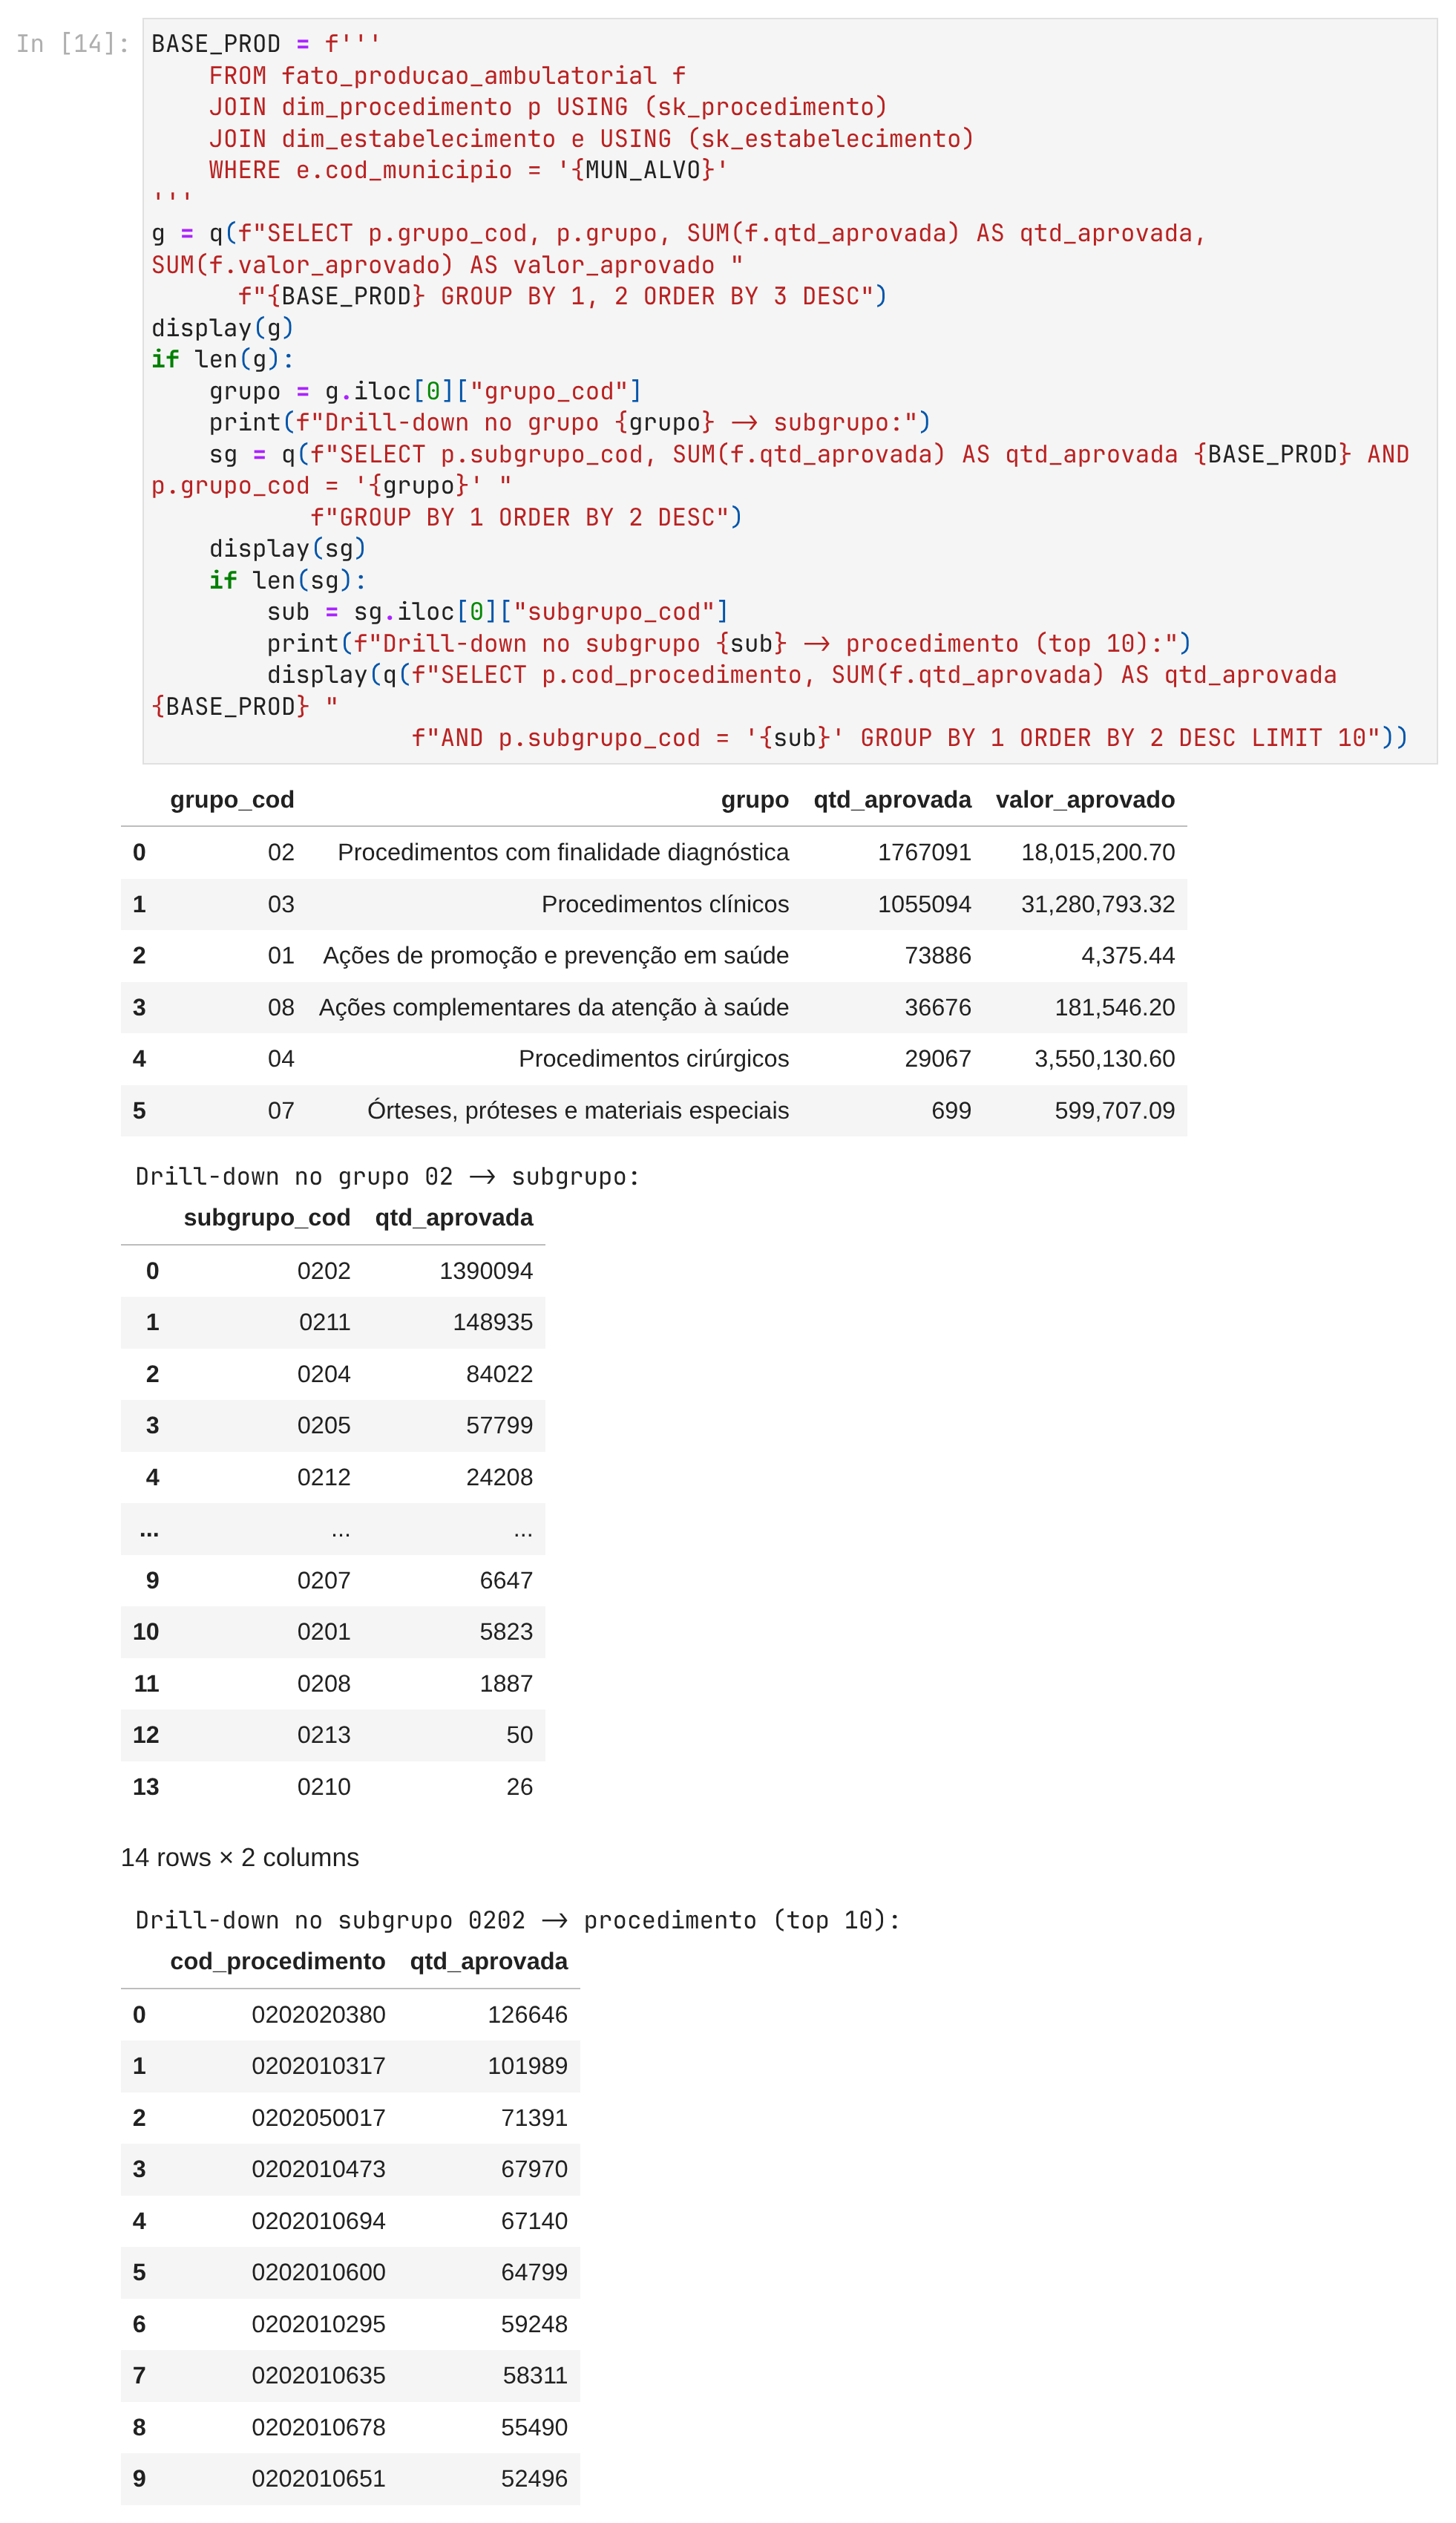
\includegraphics[width=\linewidth,height={\dimexpr\textheight-4\baselineskip\relax},keepaspectratio]{figuras/consulta2.png}
\legenda{Figura 6 – Consulta 2 no notebook: produção aprovada por grupo e drill-down até o procedimento.}
\end{figure}

\textbf{Operação OLAP:} Drill-down na dimensão procedimento (grupo → subgrupo → procedimento).


\textbf{Consulta:} Qual a quantidade aprovada de procedimentos ambulatoriais realizados em estabelecimentos de São Carlos por grupo de procedimento? Para o grupo com maior volume, detalhar por subgrupo e, para o subgrupo principal, por procedimento.


\textbf{Elementos do esquema:} Tabela de fatos: fato\_\allowbreak{}producao\_\allowbreak{}ambulatorial. Dimensões: procedimento (grupo\_\allowbreak{}cod, subgrupo\_\allowbreak{}cod, cod\_\allowbreak{}procedimento), estabelecimento (município = São Carlos). Medidas: SOMA de qtd\_\allowbreak{}aprovada e de valor\_\allowbreak{}aprovado.


\textbf{Importância e justificativa:} Mostra que tipo de atendimento a rede ambulatorial mais realiza e permite descer até os procedimentos específicos que concentram o volume e o gasto, apoiando o dimensionamento de oferta e de contratos.


\textbf{Resultado com os dados reais:} O grupo 02 (procedimentos com finalidade diagnóstica) lidera em quantidade, com 1,77 milhão de procedimentos aprovados; o grupo 03 (procedimentos clínicos) vem em segundo em quantidade, mas tem o maior valor aprovado, cerca de R\$ 31,3 milhões. Descendo no grupo 02, o subgrupo 0202 (diagnóstico em laboratório clínico) concentra 1,39 milhão, e no nível de procedimento os maiores volumes são o hemograma completo (0202020380, 126.646) e a dosagem de creatinina (0202010317, 101.989).


\FloatBarrier\subsection*{Consulta 3 – Slice and dice}\addcontentsline{toc}{subsection}{Consulta 3 – Slice and dice}

\begin{figure}[!htbp]\centering
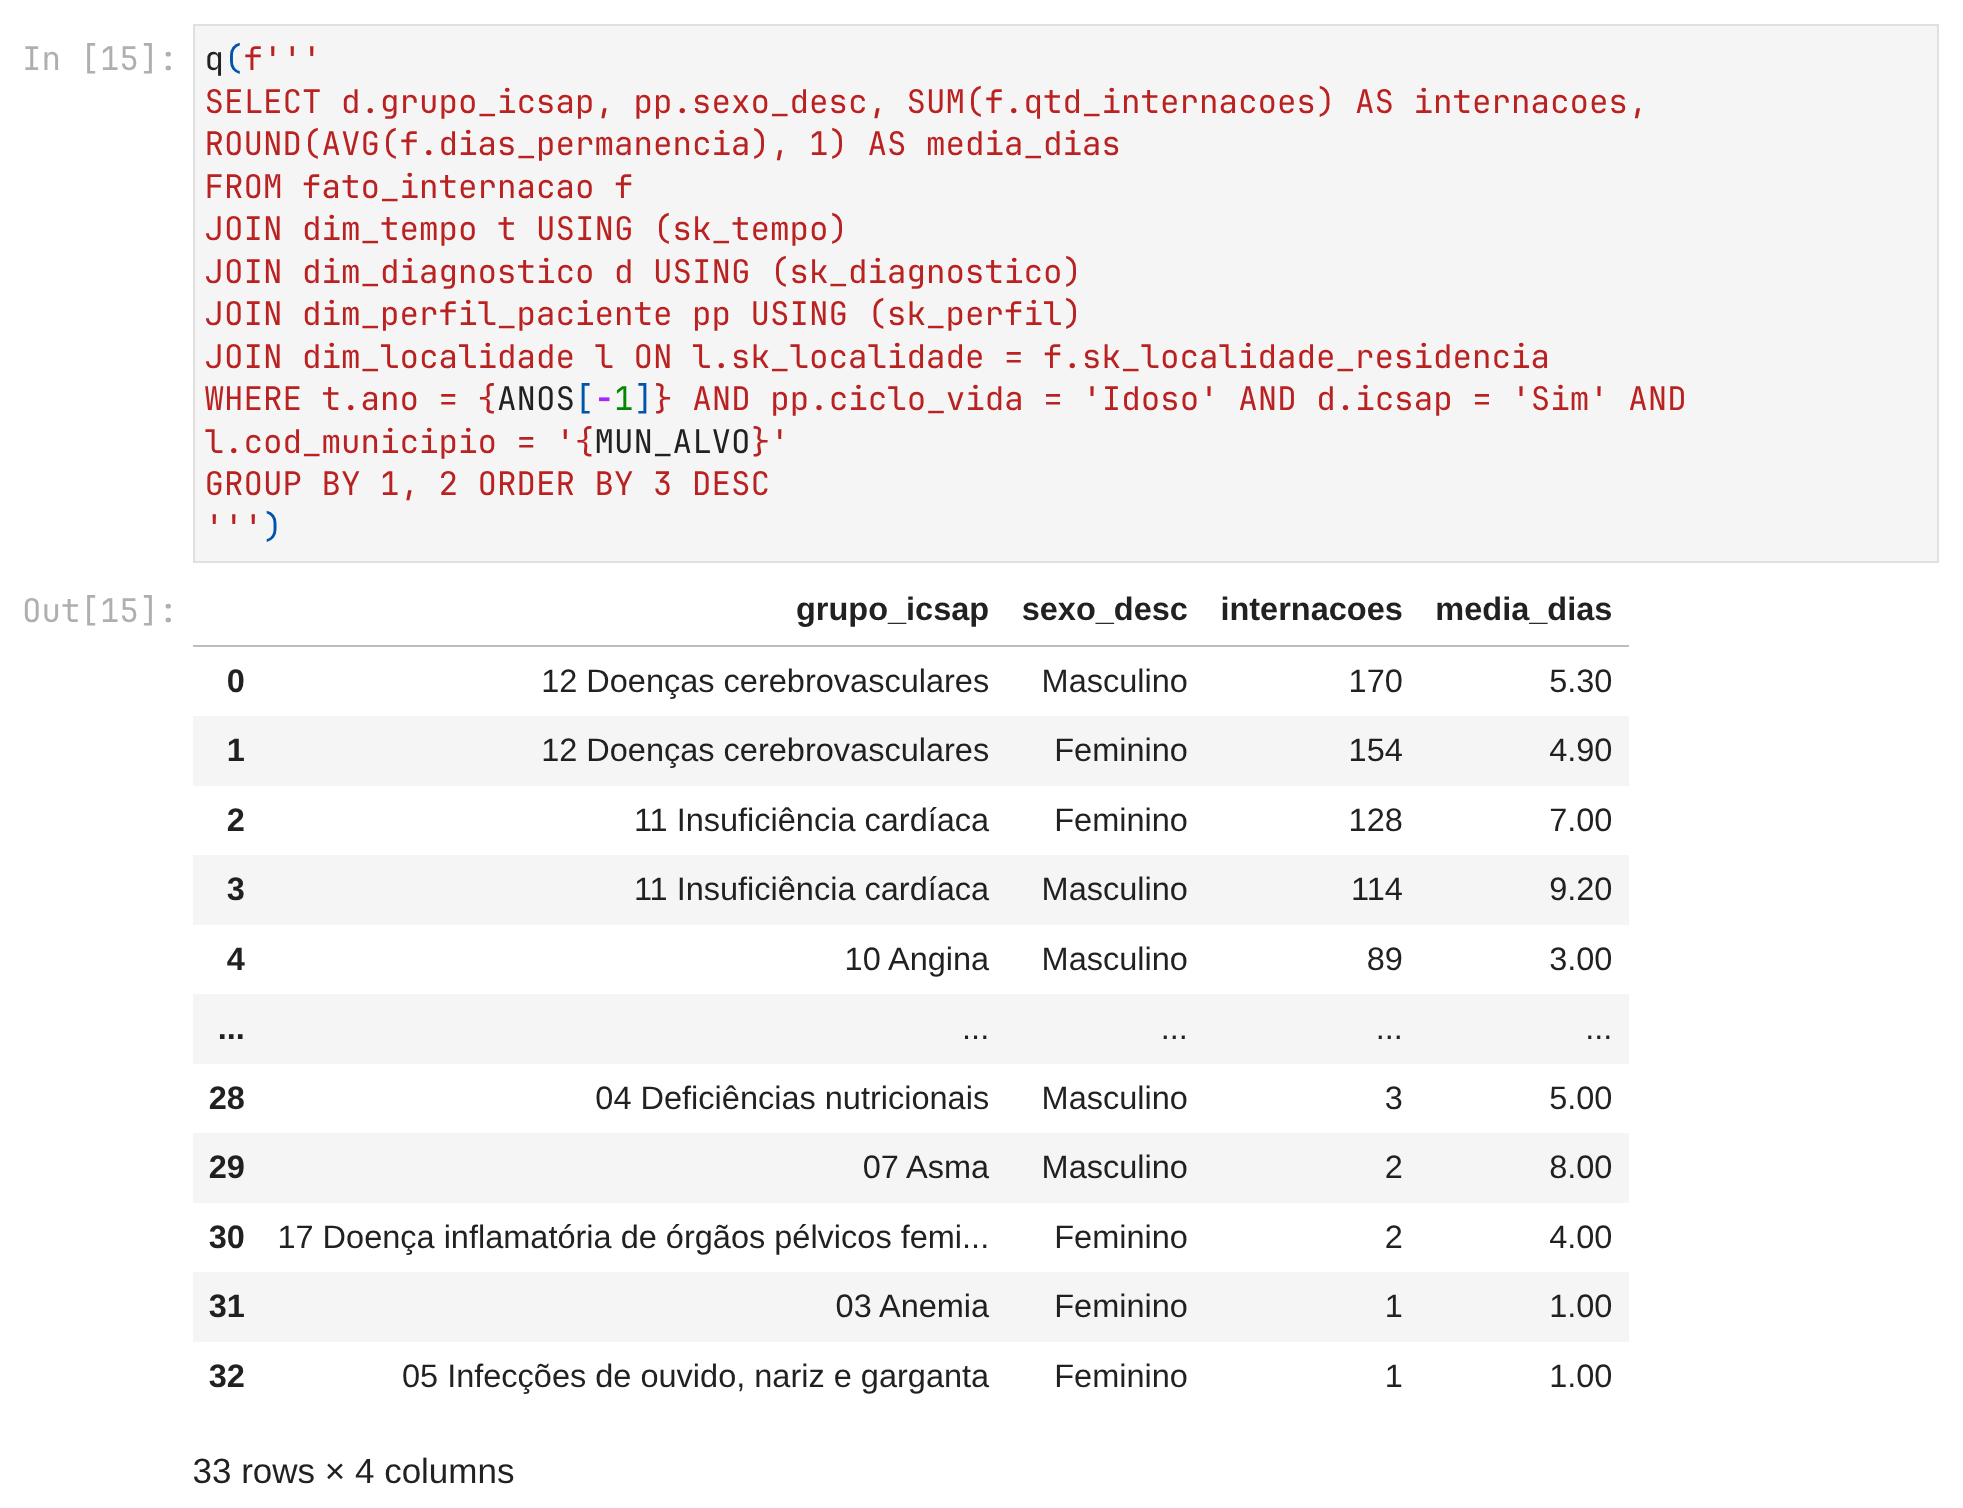
\includegraphics[width=\linewidth,height={\dimexpr\textheight-4\baselineskip\relax},keepaspectratio]{figuras/consulta3.png}
\legenda{Figura 7 – Consulta 3 no notebook: ICSAP de idosos residentes em 2024 por grupo de causa e sexo.}
\end{figure}

\textbf{Operação OLAP:} Slice na dimensão tempo (ano = 2024) e dice nas dimensões perfil do paciente (ciclo de vida = Idoso) e diagnóstico (icsap = Sim).


\textbf{Consulta:} Quantas internações por condições sensíveis à atenção primária de idosos residentes em São Carlos ocorreram em 2024, e qual a média de dias de permanência, por grupo de causa e por sexo?


\textbf{Elementos do esquema:} Tabela de fatos: fato\_\allowbreak{}internacao. Dimensões: tempo (ano), perfil do paciente (ciclo\_\allowbreak{}vida, sexo), diagnóstico (icsap, grupo\_\allowbreak{}icsap), localidade. Medidas: SOMA de qtd\_\allowbreak{}internacoes; média de permanência (derivada).


\textbf{Importância e justificativa:} Os idosos concentram as condições crônicas acompanhadas pela atenção básica, como doenças cerebrovasculares e insuficiência cardíaca. Identificar as causas que mais internam esse grupo orienta ações como grupos de hipertensos e diabéticos e visitas domiciliares.


\textbf{Resultado com os dados reais:} Foram 1.358 internações evitáveis de idosos residentes em 2024. As doenças cerebrovasculares lideram (170 homens e 154 mulheres), seguidas da insuficiência cardíaca (128 mulheres e 114 homens) e da angina (89 homens). Entre as causas mais frequentes, as doenças pulmonares e a insuficiência cardíaca têm as maiores médias de permanência.


\FloatBarrier\subsection*{Consulta 4 – Pivot}\addcontentsline{toc}{subsection}{Consulta 4 – Pivot}

\begin{figure}[!htbp]\centering
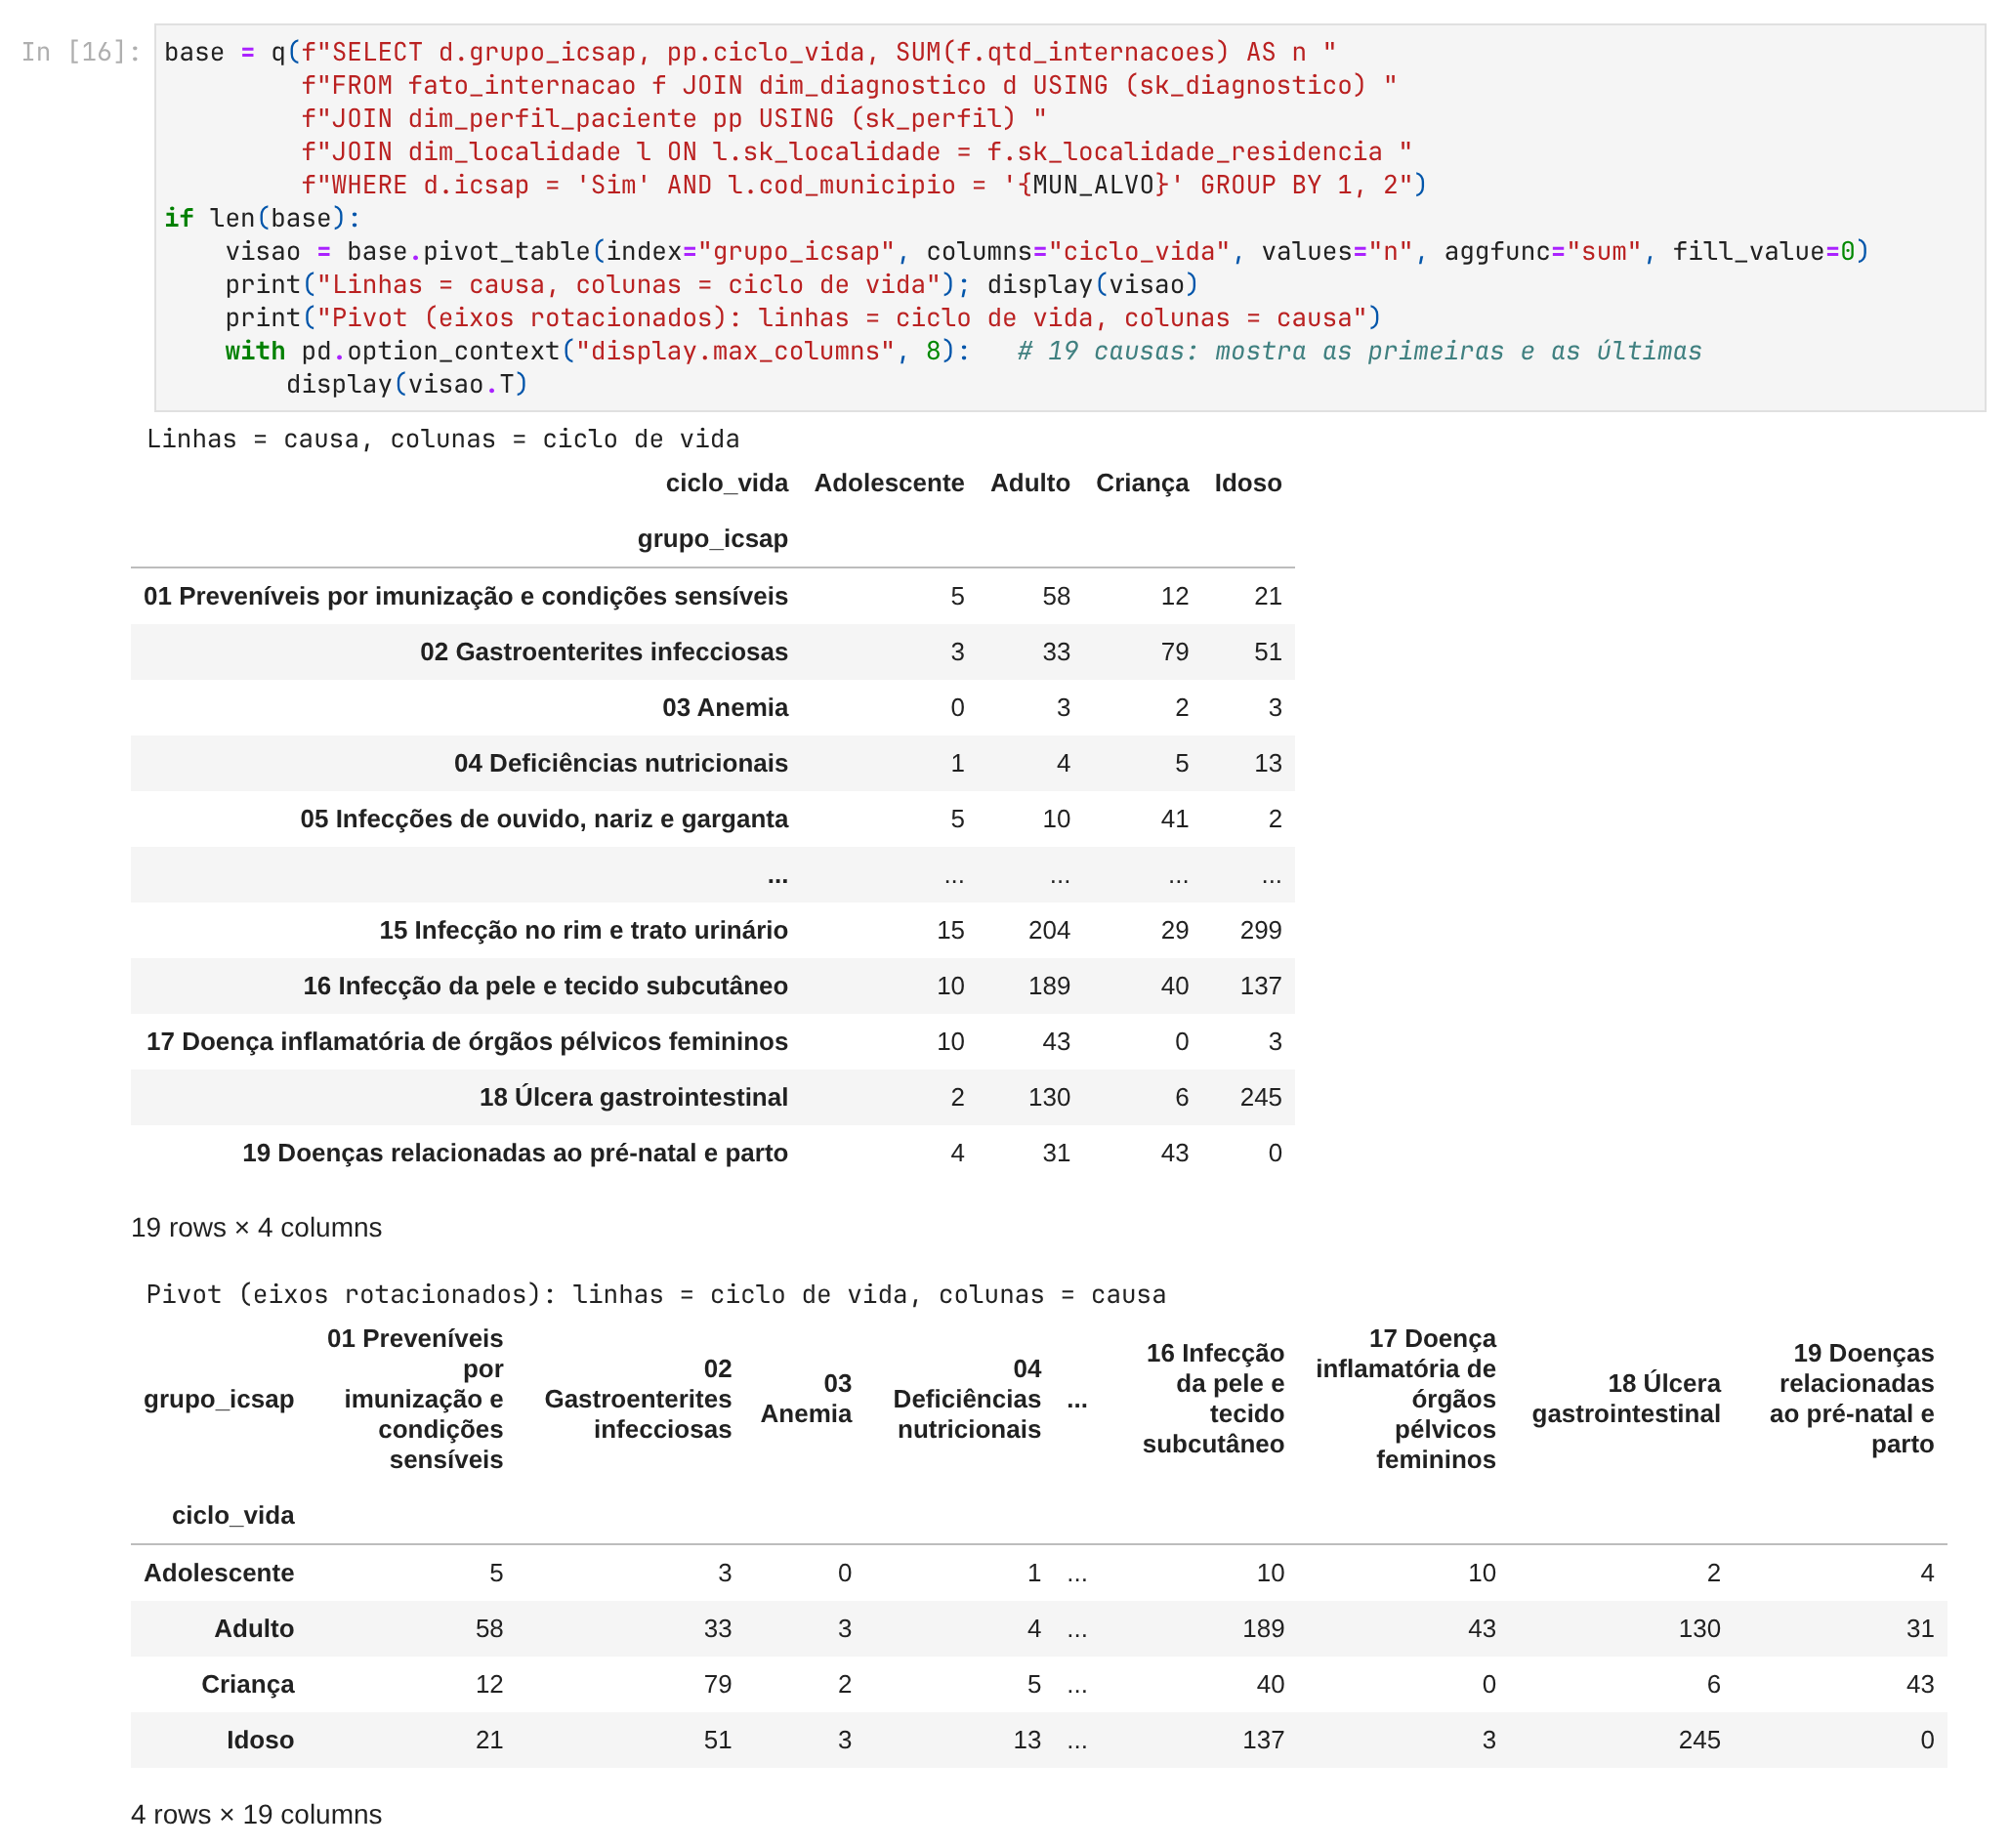
\includegraphics[width=\linewidth,height={\dimexpr\textheight-4\baselineskip\relax},keepaspectratio]{figuras/consulta4.png}
\legenda{Figura 8 – Consulta 4 no notebook: ICSAP por causa × ciclo de vida e a mesma tabela rotacionada.}
\end{figure}

\textbf{Operação OLAP:} Pivot (rotação) entre as dimensões diagnóstico e perfil do paciente.


\textbf{Consulta:} Qual o número de internações por condições sensíveis à atenção primária de residentes em São Carlos por grupo de causa (linhas) e ciclo de vida (colunas)? Em seguida, rotacionar a visão, com ciclo de vida nas linhas e grupo de causa nas colunas.


\textbf{Elementos do esquema:} Tabela de fatos: fato\_\allowbreak{}internacao. Dimensões: diagnóstico (grupo\_\allowbreak{}icsap), perfil do paciente (ciclo\_\allowbreak{}vida), localidade. Medida: SOMA de qtd\_\allowbreak{}internacoes.


\textbf{Importância e justificativa:} As duas orientações respondem perguntas diferentes do gestor: “quais causas pesam em cada fase da vida?” (útil para programas por público, como saúde da criança e do idoso) e “qual fase da vida mais sofre com cada causa?” (útil para linhas de cuidado por doença).


\textbf{Resultado com os dados reais:} Na primeira orientação, cada causa mostra em que fase da vida pesa: as doenças circulatórias são quase exclusivas de adultos e idosos (621 idosos com doença cerebrovascular nos dois anos). Na orientação rotacionada, cada fase da vida mostra suas causas: nas crianças predominam as doenças pulmonares (329) e a asma (159); nos adultos, as doenças cerebrovasculares (229), a infecção do rim e trato urinário (204) e a de pele e subcutâneo (189).


\FloatBarrier\subsection*{Consulta 5 – Drill-across}\addcontentsline{toc}{subsection}{Consulta 5 – Drill-across}

\begin{figure}[!htbp]\centering
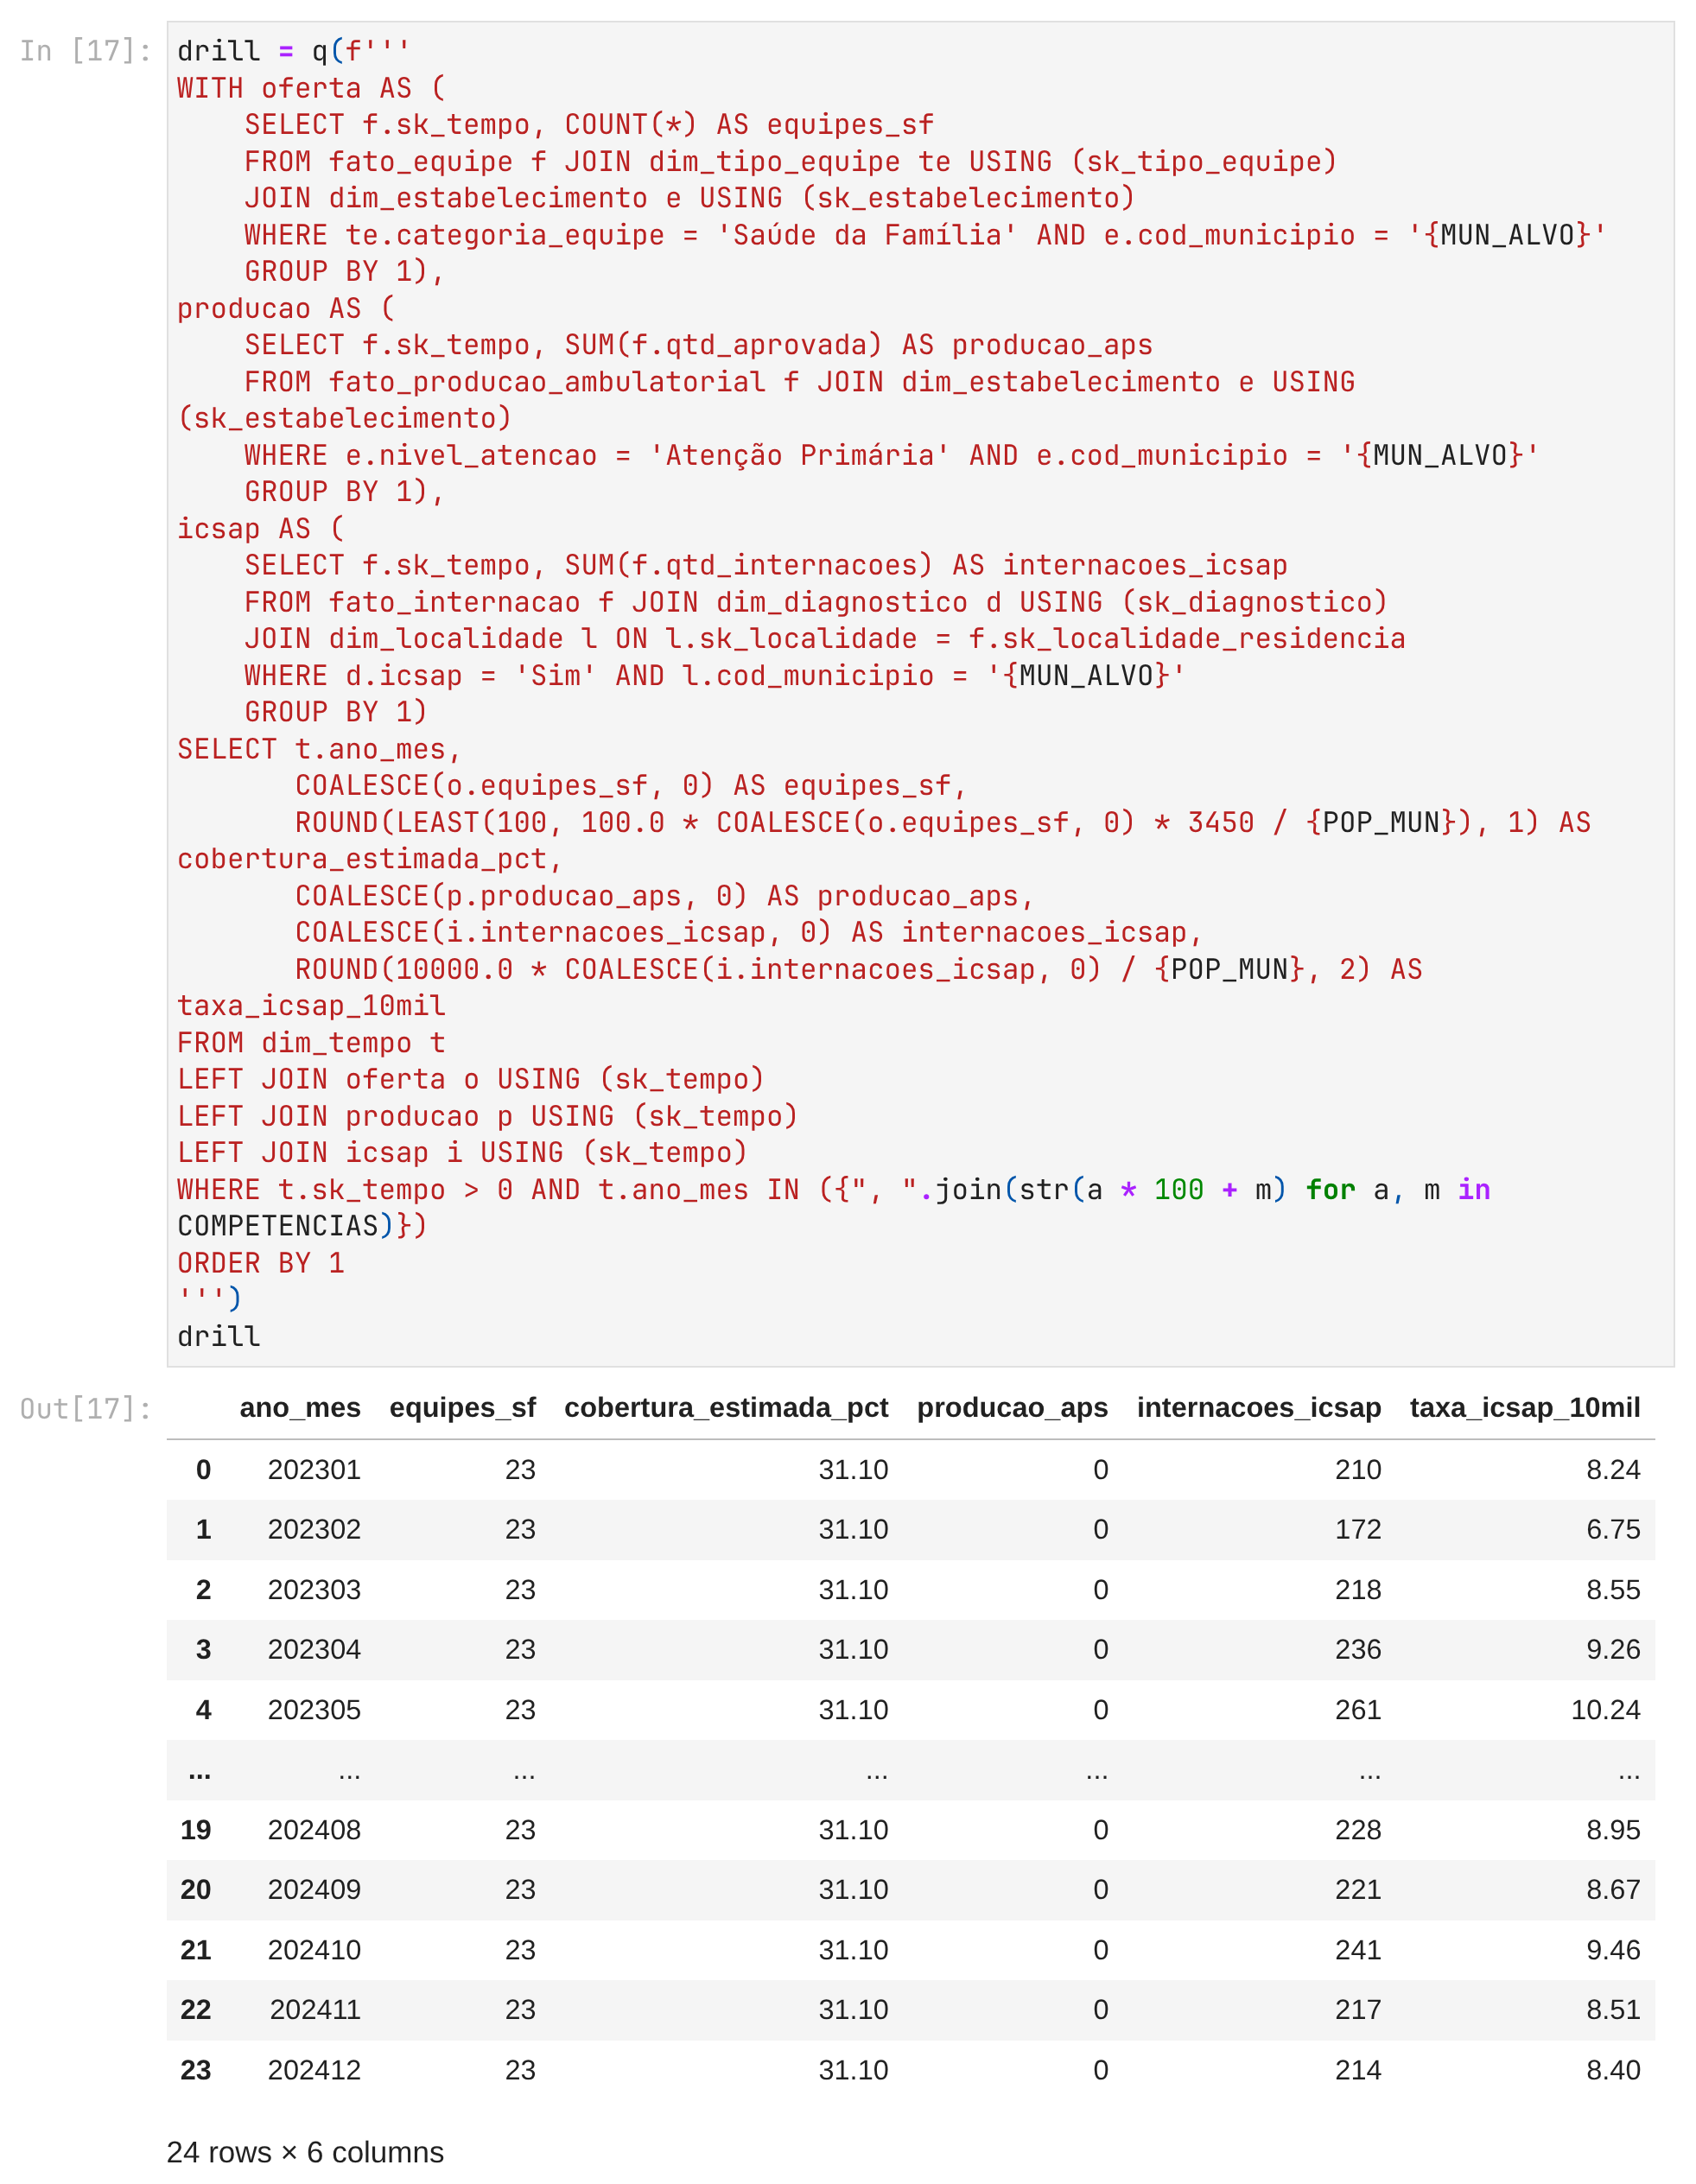
\includegraphics[width=\linewidth,height={\dimexpr\textheight-4\baselineskip\relax},keepaspectratio]{figuras/consulta5.png}
\legenda{Figura 9 – Consulta 5 no notebook: as três tabelas de fatos agregadas por mês e combinadas por ano\_\allowbreak{}mes.}
\end{figure}

\begin{figure}[!htbp]\centering
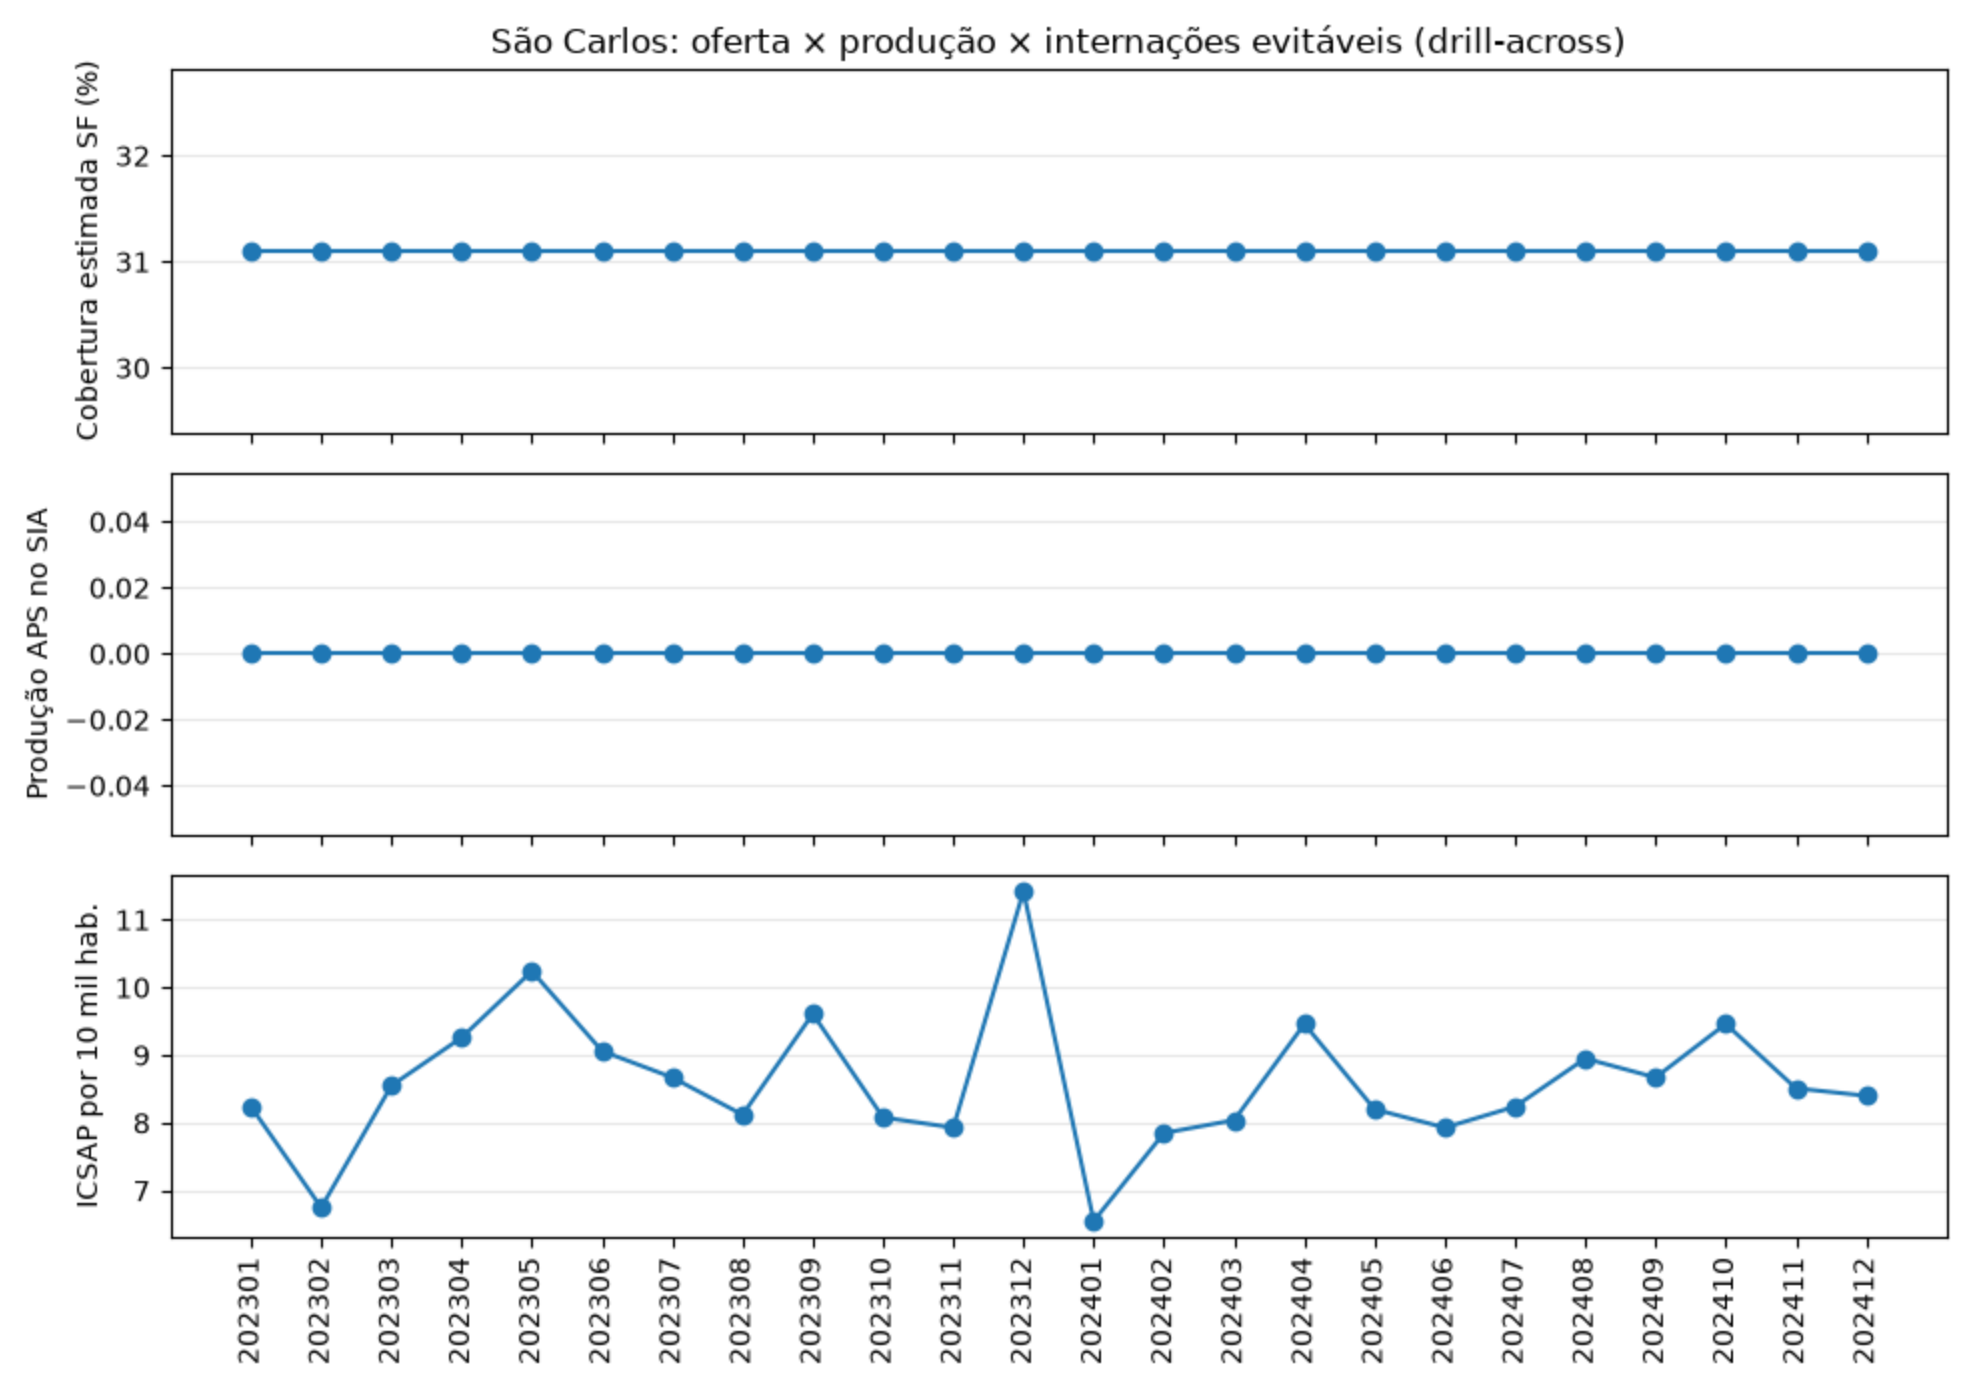
\includegraphics[width=\linewidth,height={\dimexpr\textheight-4\baselineskip\relax},keepaspectratio]{figuras/consulta5_grafico.png}
\legenda{Figura 10 – Consulta 5: resultado mês a mês, um painel por tabela de fatos com o mesmo eixo de tempo.}
\end{figure}

\textbf{Operação OLAP:} Drill-across entre fato\_\allowbreak{}equipe, fato\_\allowbreak{}producao\_\allowbreak{}ambulatorial e fato\_\allowbreak{}internacao, pela dimensão conforme tempo (e pelo município).


\textbf{Consulta:} Em cada mês, quantas equipes de Saúde da Família estavam ativas em São Carlos, qual a cobertura estimada correspondente, quantos procedimentos ambulatoriais foram aprovados nos estabelecimentos de atenção primária do município e quantas internações por condições sensíveis à atenção primária de residentes ocorreram (em número absoluto e por 10 mil habitantes)?


\textbf{Elementos do esquema:} Cada tabela de fatos é agregada separadamente por ano\_\allowbreak{}mes e os três resultados são combinados pelo mês. fato\_\allowbreak{}equipe: CONTAGEM de equipes com categoria\_\allowbreak{}equipe = Saúde da Família. fato\_\allowbreak{}producao\_\allowbreak{}ambulatorial: SOMA de qtd\_\allowbreak{}aprovada com nivel\_\allowbreak{}atencao = Atenção Primária. fato\_\allowbreak{}internacao: SOMA de qtd\_\allowbreak{}internacoes com icsap = Sim e residência = São Carlos. Medidas derivadas: cobertura estimada e taxa de ICSAP.


\textbf{Importância e justificativa:} Responde a pergunta central do trabalho: variações na oferta de atenção básica acompanham variações nas internações evitáveis? Só é possível porque as três estrelas compartilham dimensões conformes, e o resultado subsidia a decisão de expandir ou manter equipes.


\textbf{Resultado com os dados reais:} O drill-across funcionou como projetado e expôs dois fatos sobre as fontes. Primeiro, São Carlos manteve 23 equipes de Saúde da Família ativas em todos os 24 meses, o que dá cobertura estimada constante de 31,1\%. Segundo, a produção APS no SIA é zero em todos os meses, porque a produção das UBS vai para o SISAB (Seção 1.6). A taxa de ICSAP variou entre 6,55 e 11,42 por 10 mil habitantes, terminando 2024 em 8,40. Com a oferta constante no período, ainda não é possível relacionar variações de cobertura e de internações evitáveis: isso exige uma série mais longa e a inclusão do SISAB como fonte.


\FloatBarrier\subsection*{Resumo das consultas}\addcontentsline{toc}{subsection}{Resumo das consultas}

\par\noindent\begin{minipage}{\linewidth}\small\rowcolors{2}{white}{linhapar}\begin{tabular}{|>{\raggedright\arraybackslash}p{\dimexpr0.1534\linewidth-2\tabcolsep-1.33\arrayrulewidth\relax}|>{\raggedright\arraybackslash}p{\dimexpr0.2454\linewidth-2\tabcolsep-1.33\arrayrulewidth\relax}|>{\raggedright\arraybackslash}p{\dimexpr0.6012\linewidth-2\tabcolsep-1.33\arrayrulewidth\relax}|}\hline\rowcolor{azul}\color{white}\bfseries Consulta & \color{white}\bfseries Operação & \color{white}\bfseries Tabela(s) de fatos \\ \hline
1 & Roll-up & fato\_\allowbreak{}internacao \\ \hline
2 & Drill-down & fato\_\allowbreak{}producao\_\allowbreak{}ambulatorial \\ \hline
3 & Slice and dice & fato\_\allowbreak{}internacao \\ \hline
4 & Pivot & fato\_\allowbreak{}internacao \\ \hline
5 & Drill-across & fato\_\allowbreak{}equipe, fato\_\allowbreak{}producao\_\allowbreak{}ambulatorial, fato\_\allowbreak{}internacao \\ \hline\end{tabular}\end{minipage}\par\medskip

\end{document}
